\chapter{System Design and Implementation for Radiation Environments}
\label{chapter:system-design}
There are several methods that can be followed when designing systems for harsh environments, such as accelerators. While some components are radiation-hardened by design, their use in designs that need to be produced in large quantities poses significant difficulties in terms of cost, availability, and lead times. Thus, evaluation techniques have been developed at CERN, and continue to evolve, for assessing the risk of using COTS components in accelerators~\cite{coronetti_rha_system_level,ferraro_phd_thesis}.

This chapter presents the component selection process and component-level radiation tests up to the complete implementation of the two prototypes, and concludes with the firmware implementation on the MCU.

\section{Component Selection Methodology}
\label{section:component-selection-methodology}
Firstly, it is important to mention all the available component options, following the classification of Danzeca~\cite[slides 15--17]{danzeca2023developing}, namely:

\begin{itemize}
    \item \textbf{Radiation-Hardened (RH):} Electronics that have been developed, packaged, and sold to provide some level of protection against radiation in a \textit{particular environment}.
    \item \textbf{Radiation-Tolerant (RT):} Components that, while not specifically designed or manufactured with radiation-hardening processes, have demonstrated through dedicated testing an inherent ability to operate reliably under the radiation levels of a target environment.
    \item \textbf{Commercial Off-The-Shelf (COTS):} Plastic packaging, industrial or automotive grade; testing is required to evaluate their tolerance to radiation environments.
\end{itemize}

However, testing every available component on the market is not feasible. Therefore, it is necessary to use as much as possible the available knowledge or documentation of already tested components. Several organizations maintain databases of previously tested parts for this purpose, including CERN's internal R2EWG database, the European Space Agency's ESCIES database, NASA's RADHOME and NEPP databases, and the IEEE Radiation Effects Data Workshop proceedings.
There are mainly three approaches that can be followed in order to design a system~\cite[slide 17]{danzeca2023developing}. More specifically, one can:

\begin{enumerate}
    \item Select unknown COTS components from the market and perform radiation tests.
    \item Select previously tested COTS components from databases and re-test them at component level.
    \item Select and accept COTS components with existing radiation test data.
\end{enumerate}

In this thesis, a combination of the first and the third approaches is followed. The resources that are used in the scope of this work are \textit{i) the R2EWG database} and \textit{ii) radiation-tolerant developments of CERN, such as DI/OT~\cite{ratopus_jacow}}. The already tested components of the internal database usually have sufficient data from tests performed in radiation beams or environments representative of the CERN accelerator complex. Of course, as will be showcased later, a position encoder had to be selected and tested separately, as there was no such component available in the databases.

\section{Radiation Testing of Commercial Integrated Solution}

Before designing and testing the discrete radiation-tolerant system, a system-level validation was first performed using a commercial open-source BLDC driver. The board is based on the DRV8316 integrated BLDC gate driver~\cite{ti_drv8316}, the AS5047D magnetic rotary encoder~\cite{ams_as5047d}, and the SAMD21G18 ARM Cortex-M0+ microcontroller~\cite{microchip_samd21}. As will be detailed in Section~\ref{section:circuit-design}, both the AS5047D and the SAMD21G18 are also part of the final designed system, making this preliminary validation directly relevant to the target architecture.

The open-source hardware design was sourced from a publicly available repository~\cite{adinack_motor_controller}, and a SimpleFOC~\cite{simplefoc} demo application was written to implement field-oriented control for this validation step.
In addition, a custom mechanical mounting structure was designed in SOLIDWORKS and fabricated in ABS using a Bambu Lab 3D printer, in order to integrate the motor and the diametrically magnetized permanent magnet~\cite{simplefoc_magnet_placement}. The complete assembly is shown in Figure~\ref{fig:drv8316-system-solidworks}. The only critical mechanical requirement is that the magnet, mounted on the green adapter, must be coaxially aligned with the AS5047D magnetic encoder to ensure accurate rotor position readings.

\begin{figure}[H]
    \centering

    \begin{subfigure}{0.49\textwidth}
        \centering
        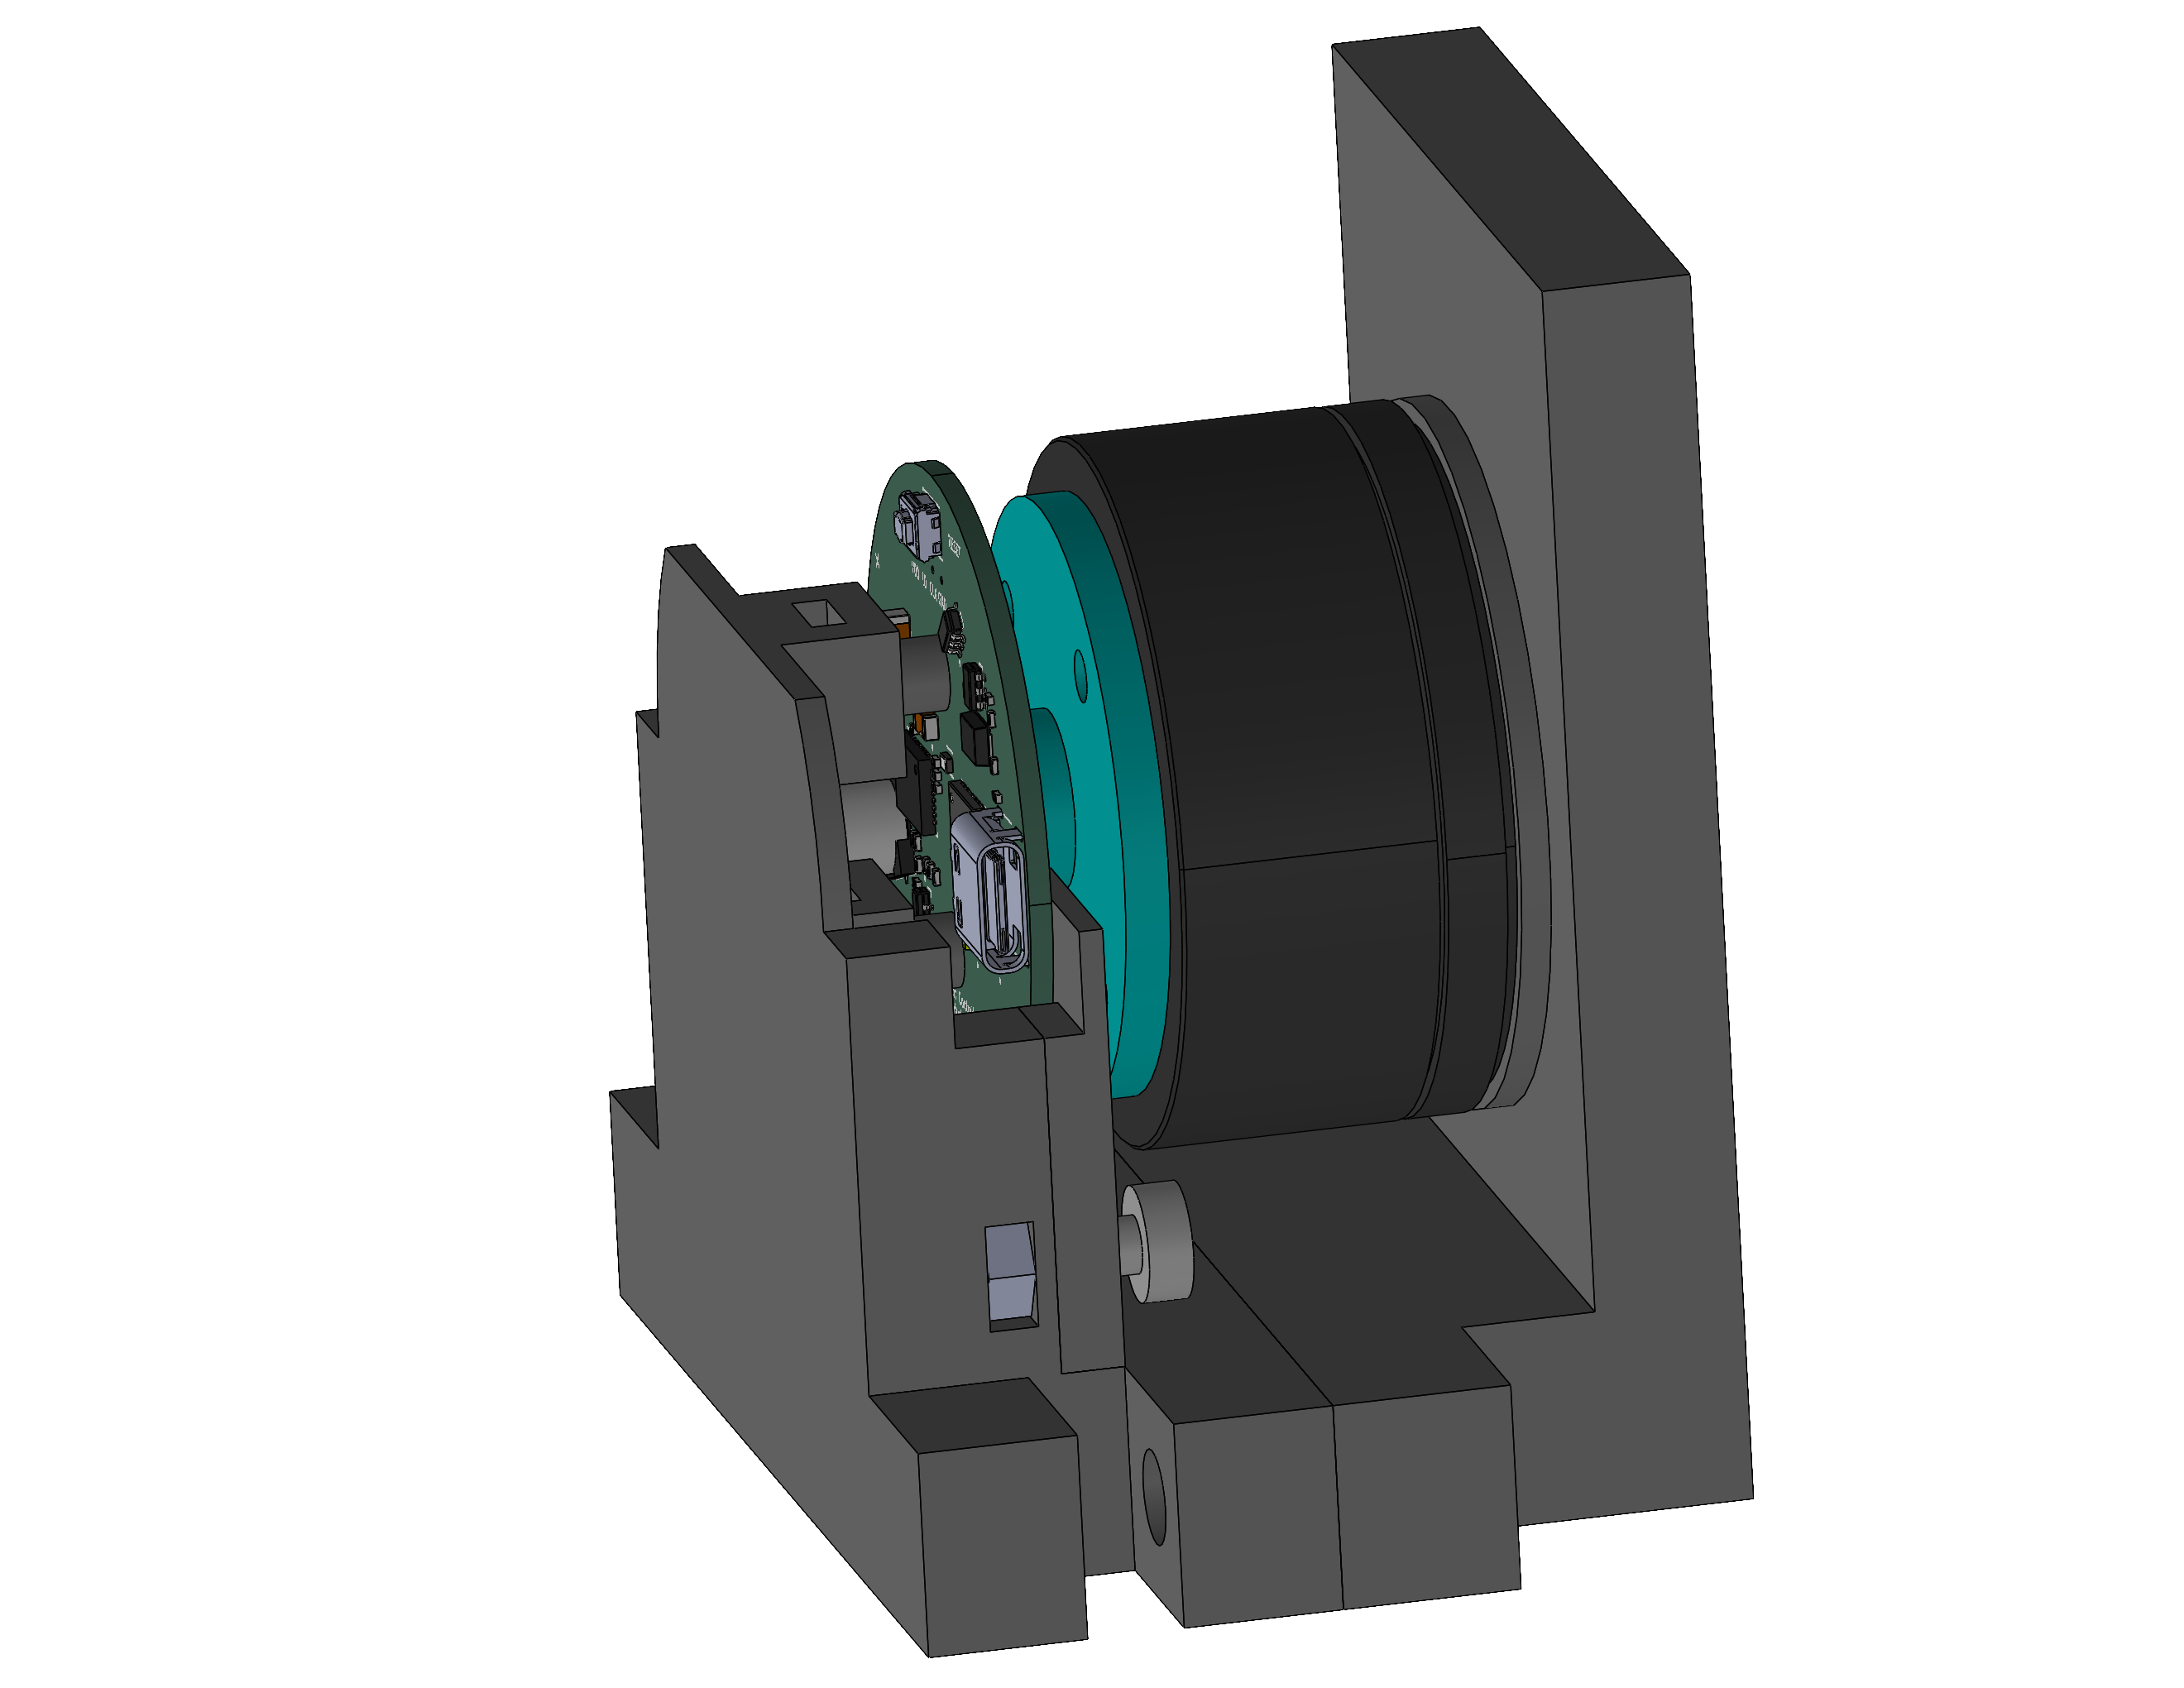
\includegraphics[width=\textwidth]{04_DesignForRadiationEnvironment/images/BLDC_Setup_Assembly.PNG}
        \caption{Panoramic view of the setup}
        \label{fig:drv8316-panoramic}
    \end{subfigure}
    \hfill
    \begin{subfigure}{0.49\textwidth}
        \centering
        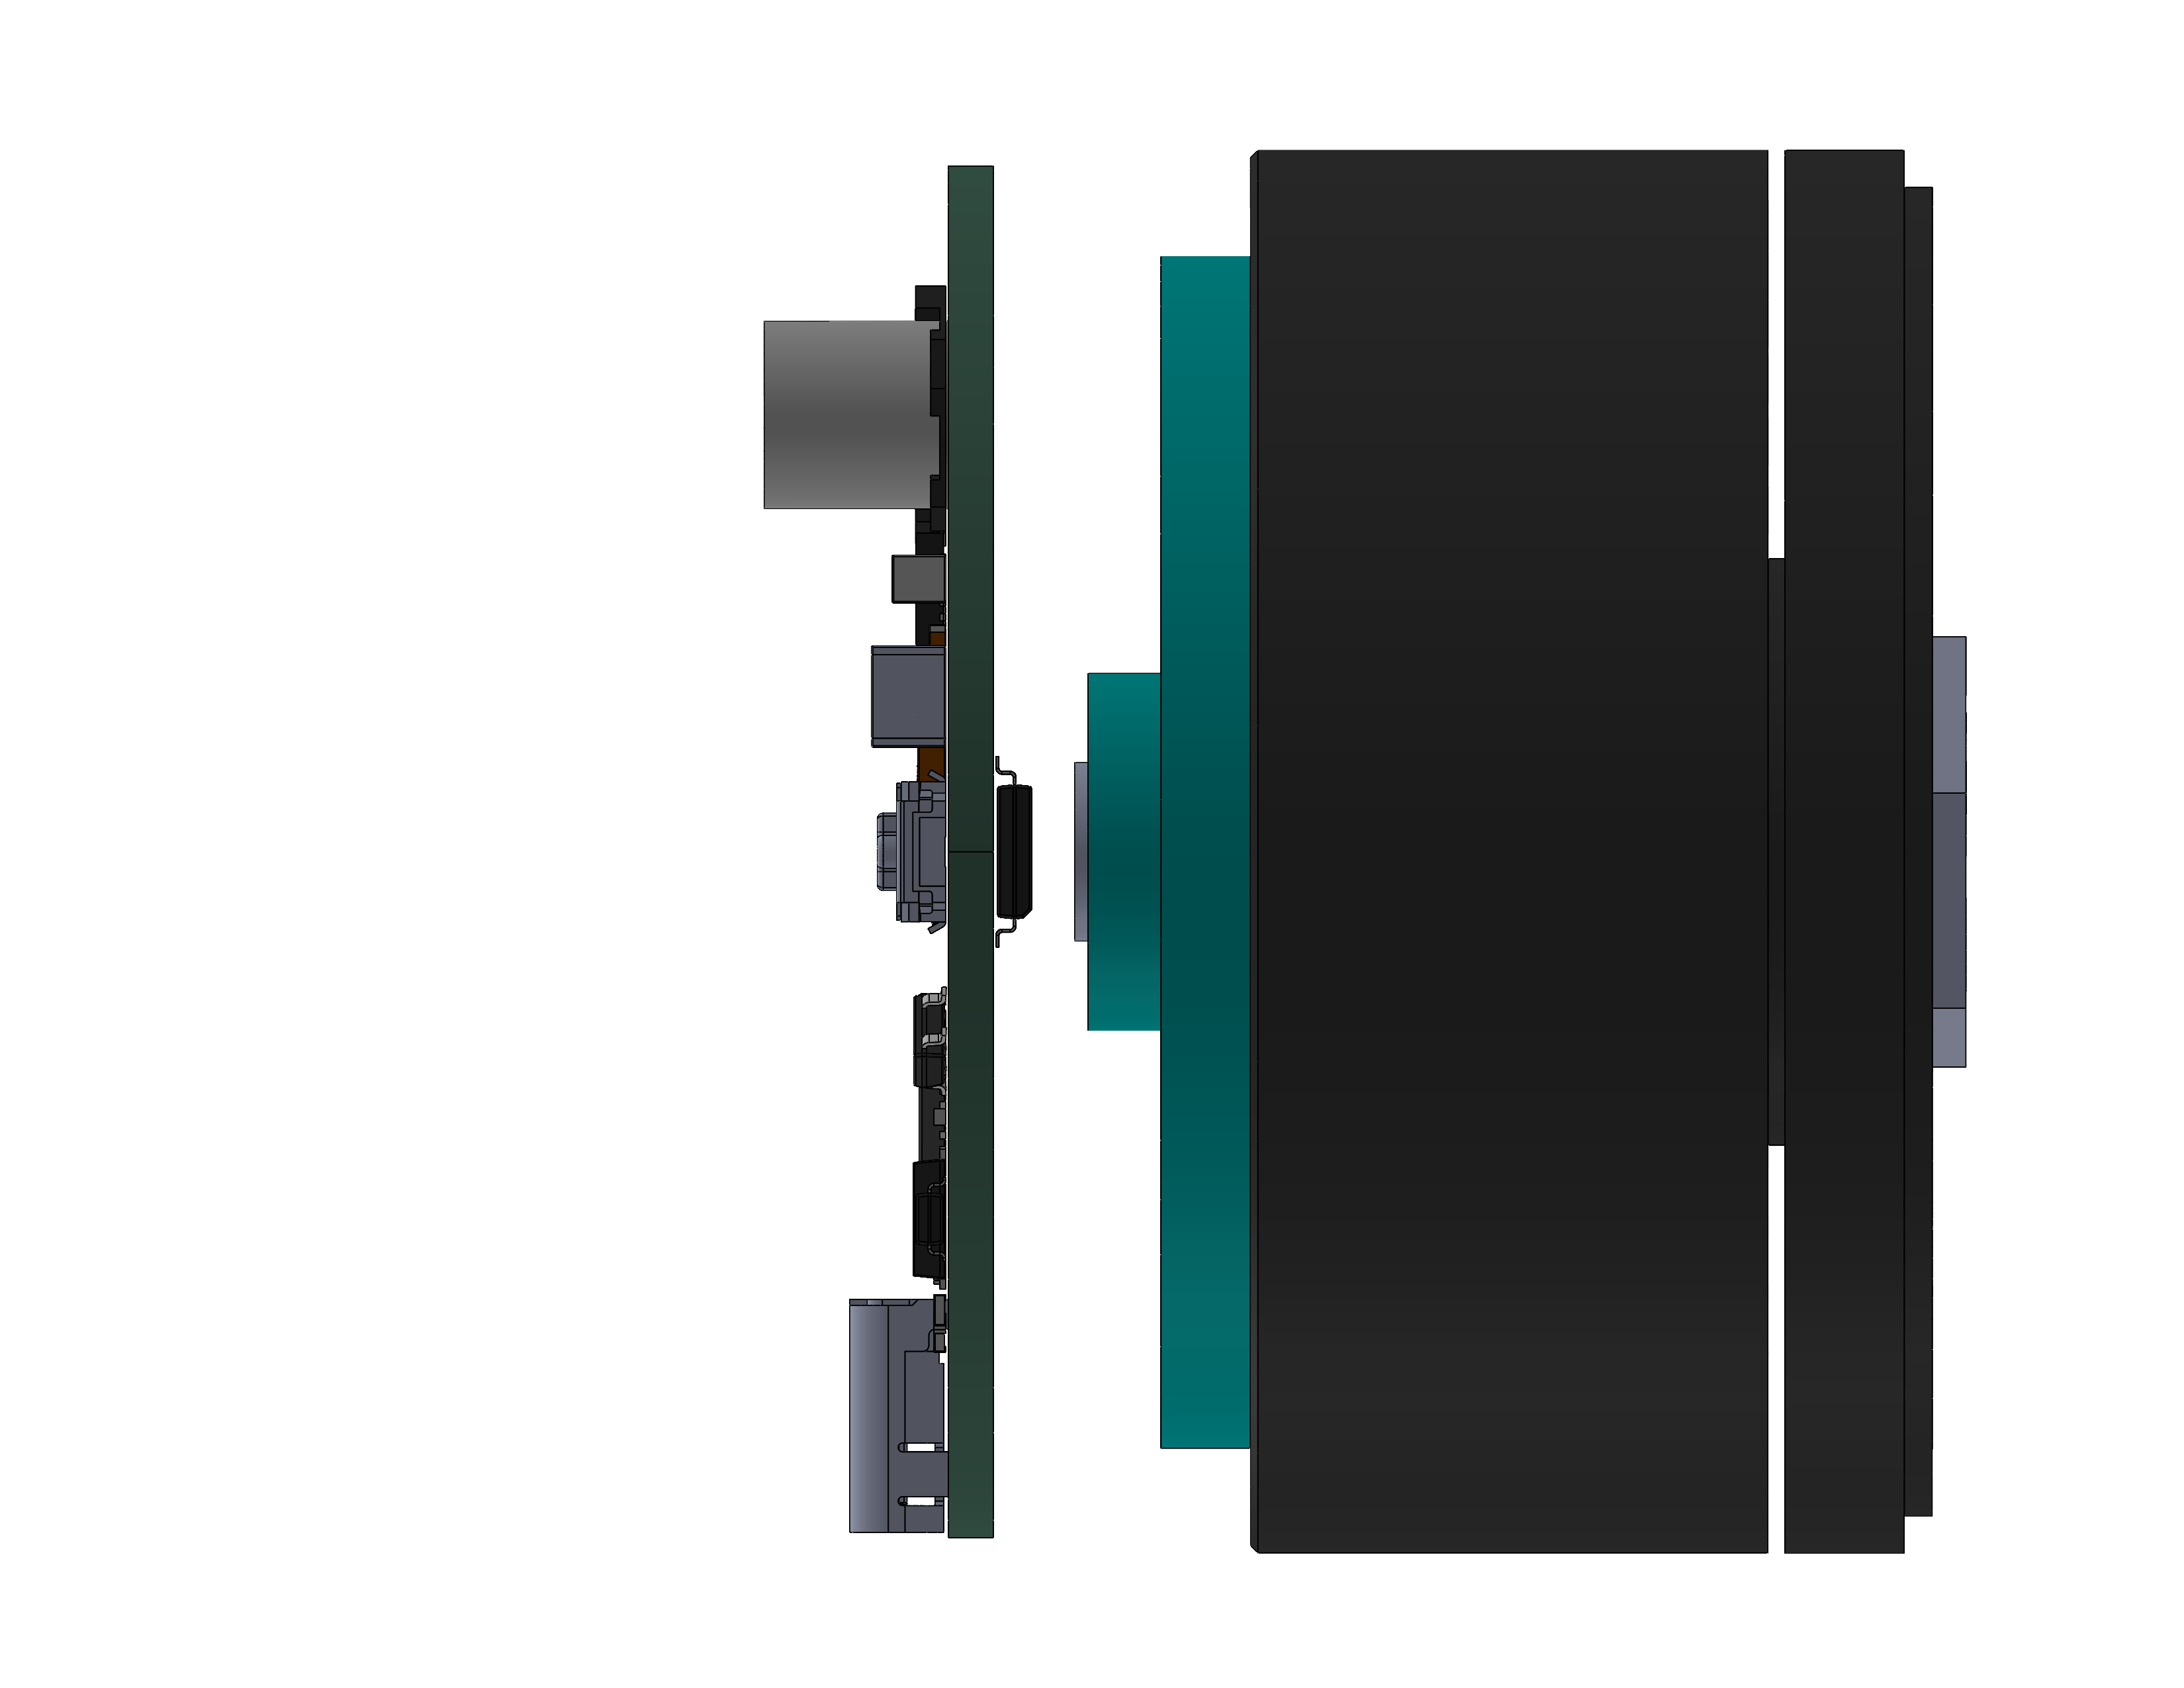
\includegraphics[width=\textwidth]{04_DesignForRadiationEnvironment/images/BLDC_Setup_Assembly-4.PNG}
        \caption{Alignment of magnet to encoder}
        \label{fig:pcb-iter-1-back}
    \end{subfigure}

    \caption{3D render of the mechanical structure that supports the test}
    \label{fig:drv8316-system-solidworks}
\end{figure}

The results of the test that took place at CHARM were particularly disappointing as the system did not survive more than 15 Gy.

\section{Components Selection and Circuits Design}
\label{section:circuit-design}

\subsection{Control Unit Selection}
A digital controller is the core of every modern motor control application and it is, actually, the factor that affects the control mostly. It is responsible for interfacing with the various analog circuits and analog/digital sensors, the operator, and of course perform all the control algorithms. Therefore, it is of great importance to select a controller that will be as robust as possible to long-term degradation (TID, DD), and to stochastic soft/hard SEE (SEL, SEU, SEFI).

Options for controllers include: microcontrollers (MCU), microprocessors (MPU), FPGA, and Digital Signal Controllers (DSC). The focus will be given to MCU and FPGA devices that have already been tested and integrated in other system designs~\cite{ratopus_jacow,toner_crome_fpga}.

In the context of the effects of radiation to electronics, the FPGA appears to be the best choice for integration in radiation tolerant design, as it provides:

\begin{enumerate}
    \item \textbf{Flexibility:} The ability to develop highly customized and complex tasks directly at the hardware level unlocks the most possibilities for high-performance control. Furthermore, hardware-level radiation-induced fault mitigation techniques can be designed, such as TMR, enabling prospect for the maximum safety
    \item \textbf{Scalability:} Available in various sizes and configurations and thus, enabling the possibility to further develop a product without the need to completely migrate to different platforms
    \item \textbf{Processing Power:} The processing power is very high compared to its counter-parts and it can be tailored to specific applications for maximum performance; ability to drive more than one motors at the same time
\end{enumerate}

On the other hand, an MCU sacrifices all of the above in exchange for ease of initial development and integration. The integrated peripherals such as ADC, TCC, USART, SPI, and TC provide enough flexibility for designing a first prototype system. Of course, the impossibility of applying mitigation techniques at the hardware level makes it necessary to implement as much as possible in software and with external hardware, like an external watchdog timer.

So, for the needs of this work, and for enhancing the development speed, the selection of the SAMD21G18A MCU was a straightforward choice~\cite[pp.~120--121]{zimmaro_phd_thesis}.

\subsection{Three-Phase Inverter}
\label{subsec:three_phase_inverter}
A three-phase inverter is typically implemented using six power switching devices arranged as three half-bridges. Depending on the voltage, current, switching-frequency, efficiency, and robustness requirements, the switching devices can be implemented using BJTs, MOSFETs, IGBTs, or more recent wide-bandgap technologies such as GaN or SiC transistors.

For this work, power MOSFETs were selected as switching devices. Compared with BJTs, MOSFETs are voltage-driven devices and can be controlled by charging and discharging the gate capacitance, instead of requiring a continuous base current, thus simplifying the driving circuitry and avoiding the radiation susceptibility issues (e.g., ELDRS) associated with BJTs~\cite{ferraro_bjt_tns}. MOSFETs are also widely used in industry and at CERN, and several candidate devices were available in the R2EWG database of radiation-tested components.

Wide-bandgap devices, such as GaN and SiC transistors, were also considered during the design phase. These technologies offer attractive switching performance, although commercial SiC MOSFETs remain susceptible to single event effects despite their good TID tolerance~\cite{martinella_sic_mosfet}, and may be suitable for future versions of the design.

\subsubsection{Power MOSFET}
\label{subsubsection:power-mosfet}

The selected device must satisfy several key requirements:

\begin{enumerate}
    \item High drain-source breakdown voltage $V_{DS,BR}$ and current $I_{DS,BR}$
    \item Low on-resistance $R_{DS,ON}$
    \item High power dissipation capability for better thermal performance
    \item Low gate charge for fast switching
    \item Gate-source threshold voltage $V_{GS,TH}$ sufficiently above signal level, since it is expected to shift toward 0 V under irradiation
\end{enumerate}

NMOS devices are preferred over PMOS counterparts due to their lower $R_{DS,ON}$, higher current capability, and better switching performance. Although PMOS devices offer simpler gate driving as high-side devices, NMOS was selected for both high- and low-side switches. The main drawback of high-side NMOS is that the gate must be driven at least $V_{GS,TH}$ above the phase-node voltage, which is addressed in the gate-drive design in subsection \ref{subsection:gate-drivers}.

The \texttt{IPB320N20N3GATMA1} was selected based on its strong ambient performance and extensive characterization over TID effects. Radiation testing showed that an average effective gate voltage applied during irradiation accelerates the reduction of $V_{GS,TH}$, driving the device toward failure considerably faster than under unbiased conditions. This is particularly critical because, as the threshold voltage approaches 0 V, the MOSFET risks never fully turning off in practice, undermining the switching behavior the converter depends on. Full test conditions and results are reported in~\cite{mosfet_edms}.

\subsection{MOSFET Gate Drivers}
\label{subsection:gate-drivers}
Driving both the high- and low-side NMOS transistors requires a bootstrap gate driver, in which the high-side gate voltage is referenced to the output phase node rather than to ground — hence the term \textit{floating} gate drive. Compared to charge-pump implementations integrated in standard ICs~\cite{ti_drv8316}, the bootstrap topology has one main limitation: it cannot operate at duty cycles approaching 100\%, since the low-side MOSFET must conduct for sufficient time to recharge the bootstrap capacitor. This is not a constraint in FOC, where such extreme duty cycles are not required.

Among the radiation-hardened components surveyed, integrated bootstrap drivers were the only viable candidates. The L6498D was selected for the first prototype; however, the device failed due to Total Ionizing Dose (TID) effects in both the CHARM and CC60 irradiation campaigns, as analyzed in Chapter~\ref{chapter:rad-tests-results}. The revised PCB was therefore designed to accommodate both the L6498D and the NCP5183, and after the latter passed radiation testing, it was adopted as the final solution.

\begin{table}[H]
    \centering
    \arrayrulecolor{thesisblue}
    \renewcommand{\arraystretch}{1.25}
    \setlength{\tabcolsep}{8pt}
    \begin{tabular}{
        >{\centering\arraybackslash}m{2.6cm}
        >{\centering\arraybackslash}m{1.8cm}
        >{\centering\arraybackslash}m{3.6cm}
        >{\centering\arraybackslash}m{2.6cm}
    }
        \rowcolor{thesisblue}
        \textcolor{white}{\textbf{Component}} &
        \textcolor{white}{\textbf{Iteration}} &
        \textcolor{white}{\textbf{Tolerant Up To (Gy)}} &
        \textcolor{white}{\textbf{Facility}} \\
        \hline
        \rowcolor{thesislightgray}
        &
        \#1 &
        &
        \\
        \rowcolor{thesislightgray}
        \multirow{-2}{=}{\centering L6498D} &
        \#2 &
        \multirow{-2}{=}{\centering 500} &
        \multirow{-2}{=}{\centering PSI} \\
        NCP5183 &
        \#2 &
        500 &
        PSI \\
        \hline
    \end{tabular}
    \caption{Radiation-tolerance test results for the selected gate drivers.}
    \label{tab:gate-driver-radiation-tolerance}
    \arrayrulecolor{black}
\end{table}

\subsection{Current Sensors}
\label{subsection:current-sensors}
Several circuit techniques exist for measuring current, the most common being shunt-resistor sensing and Hall-effect sensing. The shunt-resistor method was selected for this design, as it can be implemented with discrete components and suitable tested parts were available.

The operating principle is straightforward: the load current produces a voltage drop across a known series resistor, which is then amplified and digitized by the ADC. The shunt resistance must be chosen as a trade-off between measurement resolution and power dissipation — a larger resistance improves the signal-to-noise ratio but increases conduction losses. A generic interface between the shunt resistor, the amplifier, and the ADC is shown in Figure~\ref{fig:csa-adc-interface}.

\begin{figure}[H]
  \centering
  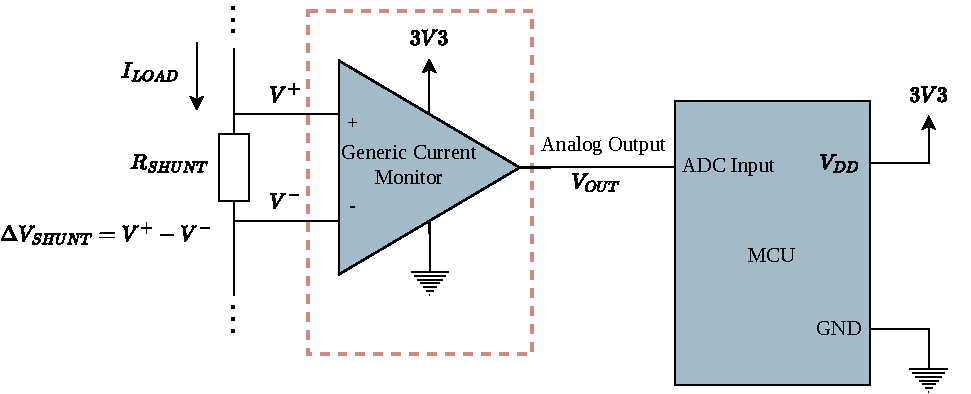
\includegraphics[width=\textwidth,keepaspectratio]{04_DesignForRadiationEnvironment/images/CSA_ADC_Interface.pdf}
  \caption{Generic interface between a shunt-based current monitor and an MCU ADC.}
  \label{fig:csa-adc-interface}
\end{figure}

For bidirectional current sensing, an offset voltage $V_{\mathrm{REF}}$ is added at the amplifier output so that both current directions can be represented within the ADC input range:

\begin{equation}
    V_{\mathrm{OUT}} = V_{\mathrm{REF}} + G \cdot R_{\mathrm{SHUNT}} \cdot I_{\mathrm{LOAD}}
\end{equation}

where $V_{\mathrm{REF}}$ is typically set close to the midpoint of the ADC input range. The current is then reconstructed in firmware as:

\begin{equation}
    I_{\mathrm{LOAD}} = \frac{V_{\mathrm{OUT}} - V_{\mathrm{REF}}}{G \cdot R_{\mathrm{SHUNT}}}
\end{equation}

\subsubsection*{Current Sensing Topology}
Three main shunt-placement topologies exist: high-side, inline, and low-side. High-side and inline sensing were both ruled out due to the common-mode voltage requirements they impose on the amplifier, which must tolerate voltages up to or exceeding the DC bus voltage. No radiation-tested component in the available database met this requirement. Low-side sensing was therefore selected.

In a three-phase PMSM control context, the preferred approach is to place one current sensor at each inverter leg, making all three phase currents directly available to the control algorithm. This reduces the computational overhead at the firmware level and increases observability, which is particularly desirable given the harsh radiation environment in which the system operates. However, low-side sensing introduces a small ground offset, cannot detect load short-circuits, and poses the greatest firmware synchronization challenge of the three topologies. Since the shunt resistor is placed between the low-side switch and ground, a clean current measurement requires both the high-side and low-side switching elements to be conducting simultaneously, creating an unambiguous current path. This condition must be mapped precisely to the correct SVPWM sector, adding complexity to the FOC implementation. The low-side topology is shown in Figure~\ref{fig:current-sense-low-side}.

\begin{figure}[H]
    \centering
    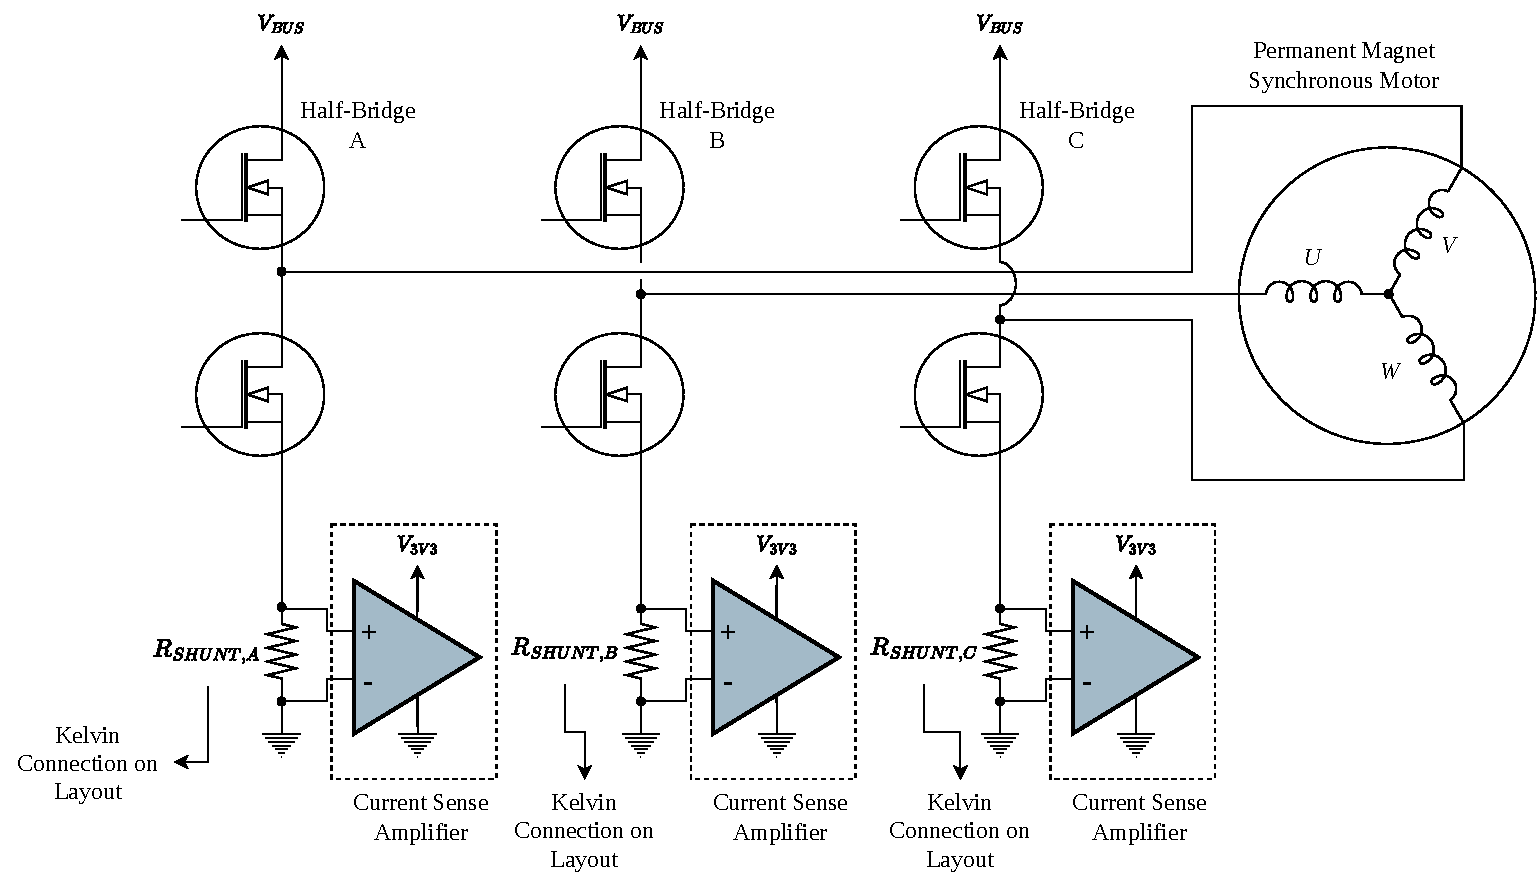
\includegraphics[width=\textwidth,keepaspectratio]{04_DesignForRadiationEnvironment/images/Current_Sense_LowSide.pdf}
    \caption{Low-side current sensing topology in a three-phase motor control application.}
    \label{fig:current-sense-low-side}
\end{figure}

\subsubsection*{Amplifier Selection}
With the low-side topology, the common-mode voltage at the shunt terminals is close to ground, which reduces the amplifier requirements considerably. Three amplifier architectures were considered: difference amplifiers, instrumentation amplifiers, and dedicated Current-Shunt Amplifiers (CSAs). The tested instrumentation amplifiers were ruled out, simply, because they were outperformed by other Op-Amps. The final choice was therefore between a discrete difference amplifier and a dedicated CSA.

\subsubsection*{Implementation}
The current-sensing circuit was subject to two design iterations, summarized in Table~\ref{tab:current_sense_iterations}. In the first iteration, a discrete difference amplifier based on the AD8030 precision operational amplifier was used. The topology is shown in Figure~\ref{fig:diff-amp-diagram}. The AD8030 had been radiation-tested up to 750~Gy with limited degradation, and the observed single-event transients were short relative to the motor-control loop timescale and therefore not expected to affect measurement quality.

\begin{figure}[H]
  \centering
  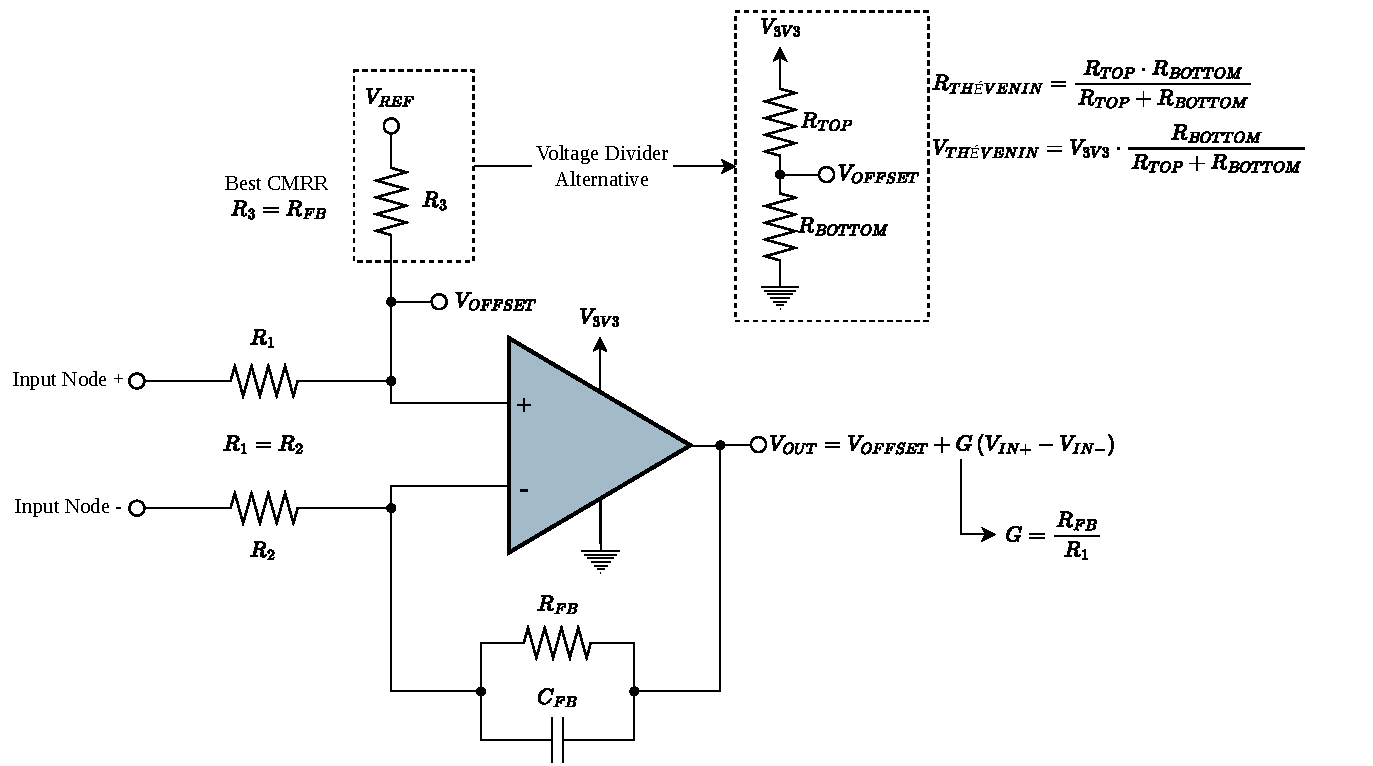
\includegraphics[width=\textwidth,keepaspectratio]{04_DesignForRadiationEnvironment/images/Difference_Amplifier.pdf}
  \caption{Difference amplifier based on a precision operational amplifier.}
  \label{fig:diff-amp-diagram}
\end{figure}

A design flaw of this design, even though it did not clearly affect the functionality, was that the offset voltage was set by a voltage divider without a voltage buffer in between. That is, except for leading to increased impedance, since the commercial resistors did not exist in values that satisfied the Thevenin equivalent with the $R_{FB}$, which led to worse CMRR, as explained in~\cite{ti_sboa551}.

In the second iteration, the discrete difference amplifier was replaced by the INA214 dedicated CSA. Compared to the discrete implementation, the INA214 offered several advantages: higher common-mode rejection due to integrated matched resistors, better rejection of switching transients, and simpler integration with the ADC. The INA214 had also been used in the CERN DIOT design, providing useful design heritage~\cite{ratopus_edms}. In the same iteration, the offset voltage generation was improved by replacing the resistors voltage divider with an ISL2109 voltage reference, resulting in equality of $R_3$ and $R_{FB}$ for optimal CMRR.

\begin{table}[H]
    \centering
    \arrayrulecolor{thesisblue}
    \renewcommand{\arraystretch}{1.25}
    \setlength{\tabcolsep}{8pt}
    \begin{tabular}{>{\bfseries\centering\arraybackslash}m{2.8cm}
                     >{\centering\arraybackslash}m{4.5cm}
                     >{\centering\arraybackslash}m{4.5cm}}
        \rowcolor{thesisblue}
        \textcolor{white}{\textbf{}} &
        \textcolor{white}{\textbf{Iteration 1}} &
        \textcolor{white}{\textbf{Iteration 2}} \\
        \hline
        \rowcolor{thesislightgray}
        Device & AD8030 & INA214 + ISL2109 \\
        Implementation & Discrete difference amplifier with voltage-divider offset & Current-shunt monitor with dedicated voltage reference \\
        \rowcolor{thesislightgray}
        Motivation & Radiation-tested discrete solution & Improved performance and integration \\
        \hline
    \end{tabular}
    \caption{Evolution of the current-sensing implementation.}
    \label{tab:current_sense_iterations}
    \arrayrulecolor{black}
\end{table}

\subsection{Position Sensor}
\label{subsection:encoders}
Since the design has to include a position sensor, in this case the design is not dictated by the component availability as there is no component like this in the databases. For that reason, the method of selecting a component without any previous data and testing it at component-level has to be used.

There are plenty of commercial position sensors in the market. The first decision is to select the type of encoder that we want; among options like magnetic, optical, capacitive, inductive, and rotary resolvers. Of course, each of the above technologies come with its own pros and cons. Furthermore, the encoders are further categorized depending on whether they are incremental or absolute.

Thus, a magnetic encoder is utilized. The main reason are the convenience of both electrical and mechanical integration and the simplicity of the communication with the MCU. In an other case, there are MCUs that support quadratic decoder peripherals that perform the decoding in hardware. In that case, an alternative position encoder could be integrated.

The selection of the AS5047P encoder was final as the results of the radiation test were decent. The test results are presented in the following section \ref{sec:encoder-rad-test}.

\subsection{Power Stage and Voltage Reference}
The radiation tolerance test results for the remaining components are summarized in Table~\ref{tab:component-radiation-tolerance}.

\begin{table}[H]
    \centering
    \arrayrulecolor{thesisblue}
    \renewcommand{\arraystretch}{1.25}
    \setlength{\tabcolsep}{8pt}
    \begin{tabular}{
        >{\centering\arraybackslash}m{2.3cm}
        >{\centering\arraybackslash}m{2.8cm}
        >{\centering\arraybackslash}m{1.6cm}
        >{\centering\arraybackslash}m{3.2cm}
        >{\centering\arraybackslash}m{2.2cm}
    }
        \rowcolor{thesisblue}
        \textcolor{white}{\textbf{Part No.}} &
        \textcolor{white}{\textbf{Component}} &
        \textcolor{white}{\textbf{Iteration}} &
        \textcolor{white}{\textbf{Tested Up To (Gy)}} &
        \textcolor{white}{\textbf{Facility}} \\
        \hline
        \rowcolor{thesislightgray}
        TPS7A4501 &
        LDO &
        \#1 &
        500 &
        PSI \\
        TPS7A4901 &
        LDO &
        \#2 &
        722 &
        CHARM, PSI \\
        \rowcolor{thesislightgray}
        ISL2109 &
        Voltage Reference &
        \#2 &
        500 &
        PSI \\
        TPL5010 &
        WDT &
        \#2 &
        300 &
        -- \\
        \hline
    \end{tabular}
    \caption{Radiation test results summary for the selected components.}
    \label{tab:component-radiation-tolerance}
    \arrayrulecolor{black}
\end{table}

The external watchdog TPL5010 was adopted from BatMon, an in-house radiation monitoring system used in particle accelerators~\cite{batmon, batmon_edms}. However, as shown in Chapter~\ref{chapter:rad-tests-results}, the external WDT did not survive beyond 300 Gy and was therefore excluded from the final test.

Regarding the TPS7A4901 LDO, beyond the numerous tests that have been performed, it is also used in the design of the DC/DC stage of RaToPUS, a radiation-tolerant power supply~\cite{ratopus_jacow,ratopus_edms,ratopus_ohwr}.

\section{Radiation Testing of a Magnetic Encoder}
\label{sec:encoder-rad-test}

The test took place at the PSI PIF facility. The objective of the test was to evaluate the behavior of the magnetic encoder under proton beam irradiation.

\subsection{Test Procedures \& Setup}

The first step before performing the test was to define the setup and the test procedures. The device was tested using its SPI interface and without the internal LDO, with the Dynamic Angle Error Compensation (DAEC) feature enabled, and the setup consisted of the an AS5047P evaluation board, a Feather-M0+ breakout board by Adafruit, and a magnet holder.

For the scope of this test, no motor was needed as it would add the extra complexity of driving electronics and would need another independent reference to compare the values. The idea in which the tested was based on was to keep the magnet mounted at the same position throughout the test. This is the most deterministic way of evaluation as the rotation is always 0 degrees and essentially the \textbf{repeatability} is under evaluation.

\begin{figure}[H]
  \centering
  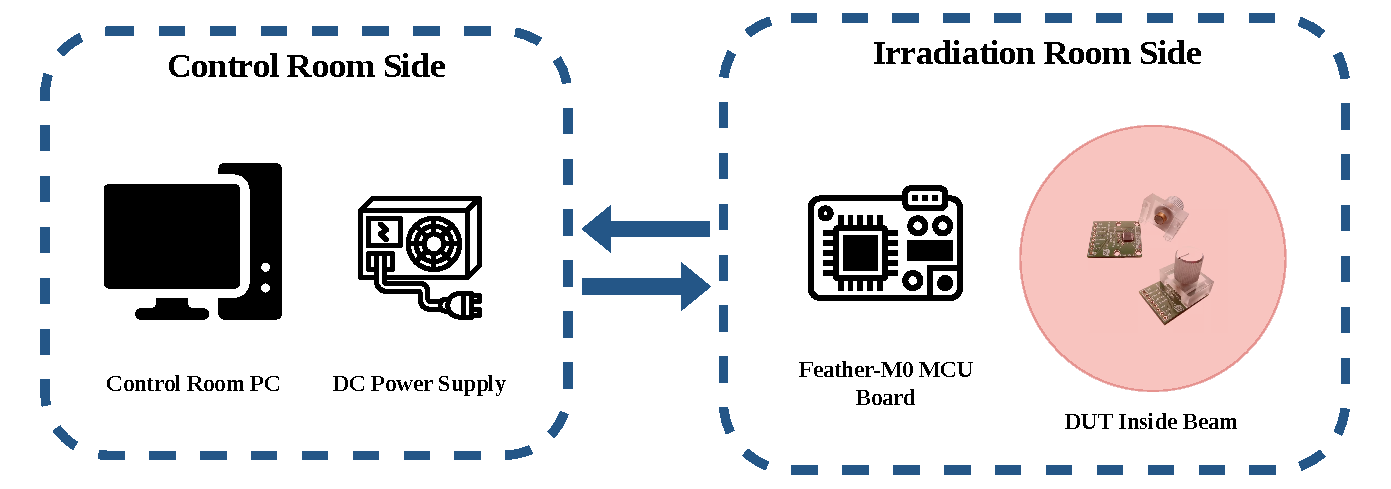
\includegraphics[width=\textwidth,keepaspectratio]{04_DesignForRadiationEnvironment/images/AS5047P_PSI_Setup.drawio.pdf}
  \caption{Setup for PSI radiation testing campaign}
  \label{fig:as5047p-psi-setup}
\end{figure}

As shown in the figure above, the MCU and AS5047P are kept inside the irradiation room and while the DUT is inside the beam, the Feather-M0+ board is kept approximately 1.5m away from it so that it is not affected by the radiation. From the irradiation room, there are two cables, one coaxial BNC for the powering of the devices (power and return) and one USB for reading the serial port from the MCU. The software that was used for this test was the open-source SimpleFOC library which implements a basic driver for the AS5047P device.

\subsection{Irradiation Runs \& Dosimetry}

According to the irradiation procedures, each irradiation run was set to \SI{100}{\gray}, after which the beam was closed, the DUT power cycled, and the beam subsequently turned on again. The same procedure was followed in the event of an SEL occurrence. The 1\,MeV\,$n_\text{eq}$ DDEF metric is used to quantify the displacement damage dose.

The DUTs were irradiated up to a TID of \SI{1}{\kilo\gray} and a DDEF of \SI{1.70e12}{\per\cm\squared} (1\,MeV\,$n_\text{eq}$), with a beam proton fluence of \SI{1.73e12}{\per\cm\squared}.

\subsection{Experimental Results}

The device was irradiated up to a total dose of \SI{1}{\kilo\gray}. The current consumption remained close to nominal throughout the irradiation, with no increasing trend observed, averaging approximately \SI{6}{\milli\ampere}, as shown in Figure~\ref{fig:as5047p-psi-current}.

\begin{figure}[H]
  \centering
  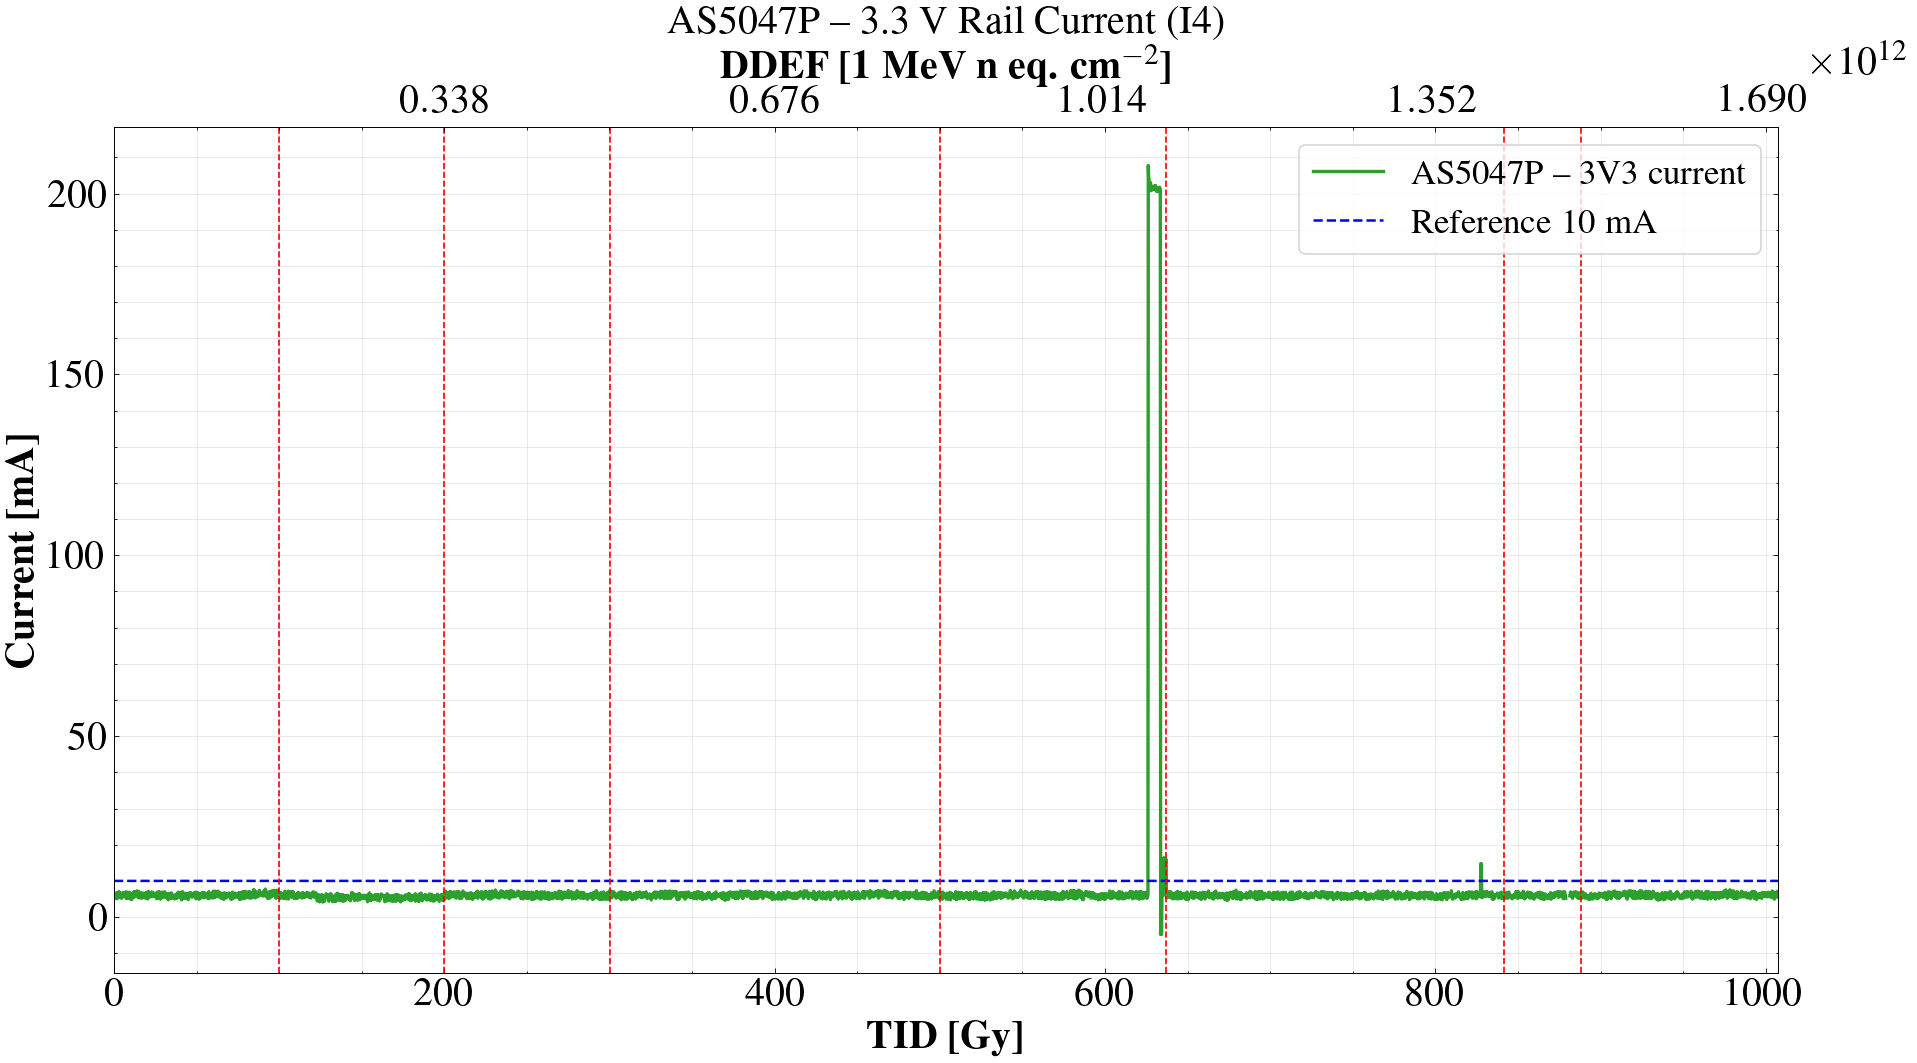
\includegraphics[width=0.9\textwidth,keepaspectratio]{04_DesignForRadiationEnvironment/images/Current_AS5047P_3V3_over_TID.png}
  \caption{AS5047P current consumption throughout the irradiation test.}
  \label{fig:as5047p-psi-current}
\end{figure}

A single SEL event was observed after a total particle fluence of \SI{1.0953e12}{\per\cm\squared}, as indicated by the PSU current exceeding the \SI{200}{\milli\ampere} protection limit. Following the event, the DUT was power cycled and fully recovered its functionality.

Regarding measurement performance, the device experienced periods of elevated noise during the first and second irradiation runs, as visible in Figure~\ref{fig:as5047p-psi-angles}. This instability was resolved following the subsequent power cycles; however, its root cause could not be determined from the available data.

\begin{figure}[H]
  \centering
  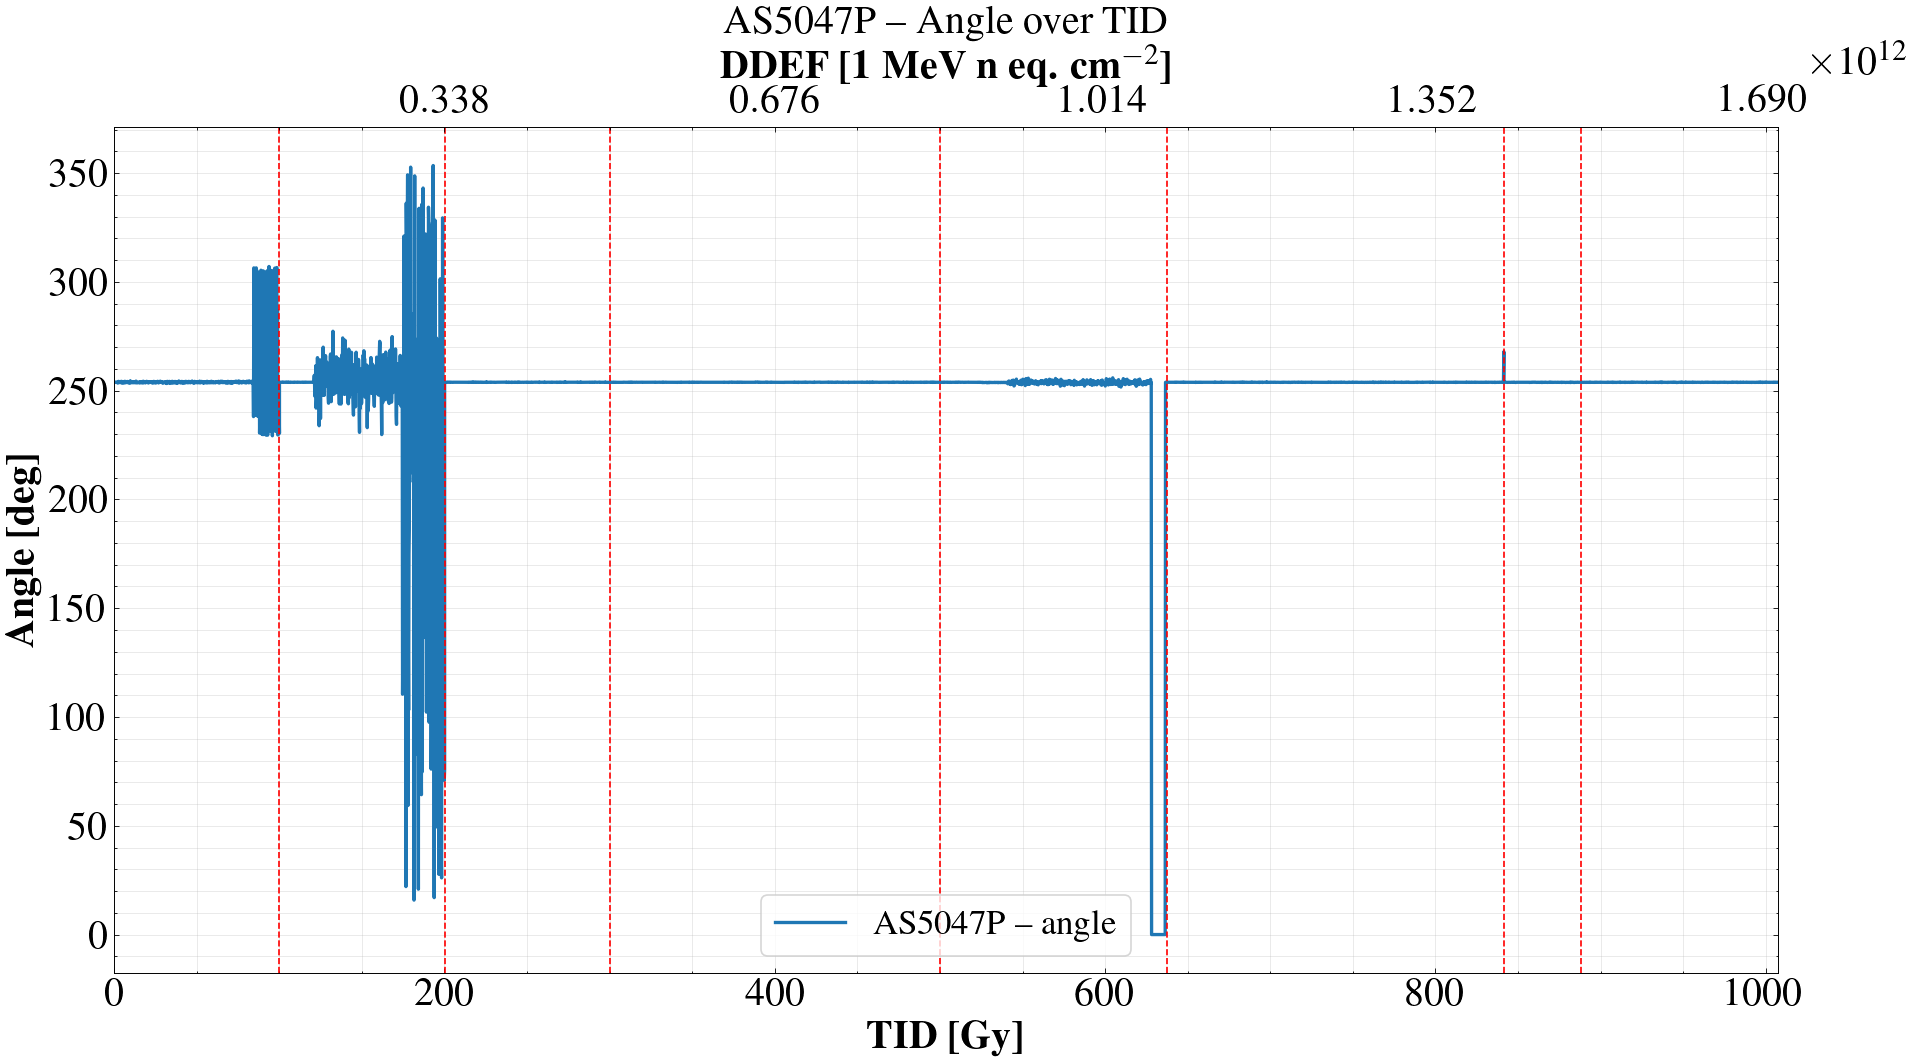
\includegraphics[width=0.9\textwidth,keepaspectratio]{04_DesignForRadiationEnvironment/images/Angle_AS5047P_over_TID.png}
  \caption{AS5047P angle readings throughout the irradiation test.}
  \label{fig:as5047p-psi-angles}
\end{figure}

To characterize the measurement performance across irradiation runs, the mean, standard deviation, minimum, and maximum of the angle readings are calculated per run. Samples acquired during the SEL event, where the output was latched to \SI{0}{\degree}, are excluded from the analysis to avoid biasing the statistics. The results are presented in Table~\ref{tab:angular-statistics-per-run}, and the corresponding precision and accuracy relative to the pre-irradiation baseline are summarized in Table~\ref{tab:precision-accuracy-relative-pre-irradiation}.

\begin{table}[H]
    \centering
    \arrayrulecolor{thesisblue}
    \renewcommand{\arraystretch}{1.25}
    \setlength{\tabcolsep}{9pt}
    \begin{tabular}{>{\bfseries}c
                    S[table-format=3.2]
                    S[table-format=2.2]
                    S[table-format=3.2]
                    S[table-format=3.2]}
        \rowcolor{thesisblue}
        \textcolor{white}{\textbf{Run}} &
        {\textcolor{white}{\textbf{Mean (\si{\degree})}}} &
        {\textcolor{white}{\textbf{Std.\ (\si{\degree})}}} &
        {\textcolor{white}{\textbf{Min (\si{\degree})}}} &
        {\textcolor{white}{\textbf{Max (\si{\degree})}}} \\
        \hline
        \rowcolor{thesislightgray}
        43 & 255.61 & 13.39 & 229.28 & 307.09 \\
        44 & 239.66 & 53.36 & 15.84  & 353.50 \\
        \rowcolor{thesislightgray}
        45 & 253.88 & 0.03  & 253.78 & 253.96 \\
        46 & 253.87 & 0.03  & 253.78 & 253.96 \\
        \rowcolor{thesislightgray}
        47 & 253.77 & 0.59  & 251.67 & 255.92 \\
        48 & 253.88 & 0.46  & 253.76 & 267.91 \\
        \rowcolor{thesislightgray}
        49 & 253.86 & 0.03  & 253.76 & 253.96 \\
        50 & 253.86 & 0.03  & 253.76 & 253.96 \\
        \hline
        \rowcolor{thesislightgray}
        Overall (43--50) & 252.59 & 18.10 & 15.84  & 353.50 \\
        Post-irradiation & 253.85 & 0.03  & 253.78 & 253.94 \\
        \rowcolor{thesislightgray}
        Pre-irradiation  & 253.89 & 0.04  & 253.81 & 253.96 \\
        \hline
    \end{tabular}
    \caption{Angular measurement statistics per irradiation run.}
    \label{tab:angular-statistics-per-run}
    \arrayrulecolor{black}
\end{table}

\begin{table}[H]
    \centering
    \arrayrulecolor{thesisblue}
    \renewcommand{\arraystretch}{1.25}
    \setlength{\tabcolsep}{12pt}
    \begin{tabular}{>{\bfseries}c
                    S[table-format=2.3]
                    S[table-format=1.3]}
        \rowcolor{thesisblue}
        \textcolor{white}{\textbf{Run}} &
        {\textcolor{white}{\textbf{\%RSD}}} &
        {\textcolor{white}{\textbf{\%Error vs.\ Pre (accuracy)}}} \\
        \hline
        \rowcolor{thesislightgray}
        43 & 5.28  & 0.677 \\
        44 & 22.65 & 5.605 \\
        \rowcolor{thesislightgray}
        45 & 0.012 & 0.004 \\
        46 & 0.012 & 0.008 \\
        \rowcolor{thesislightgray}
        47 & 0.232 & 0.047 \\
        48 & 0.181 & 0.004 \\
        \rowcolor{thesislightgray}
        49 & 0.012 & 0.012 \\
        50 & 0.012 & 0.012 \\
        \hline
        \rowcolor{thesislightgray}
        Overall (43--50) & 7.16  & 0.511 \\
        Post-irradiation & 0.012 & 0.016 \\
        \rowcolor{thesislightgray}
        Pre-irradiation  & 0.016 & 0.000 \\
        \hline
    \end{tabular}
    \caption{Precision and accuracy relative to the pre-irradiation baseline.}
    \label{tab:precision-accuracy-relative-pre-irradiation}
    \arrayrulecolor{black}
\end{table}

The results indicate that, with the exception of runs 43 and 44, the device maintained stable and accurate angle readings throughout the irradiation, with post-irradiation performance essentially identical to the pre-irradiation baseline. The SEL upper limit cross-section, calculated with a 95\% confidence level Poisson upper limit, is $\sigma_\text{upper} = \SI{3.22e-12}{\cm\squared}$.

It is important to note that the PSI proton irradiation tests are not fully representative of the LHC radiation environment at CERN. The dose rates at PSI are significantly higher than those encountered at LHC positions where COTS components are typically deployed, and the DD/TID ratio differs considerably from that of the LHC mixed field. These results should therefore be interpreted as a component-level screening test rather than a full radiation qualification. Nevertheless, the device demonstrated sufficient tolerance to be considered a viable candidate for integration into the first system prototype.

\section{Final Hardware System Design}
\label{sec:final-hardware-overview}

\subsection{Rad-Tol Motor Controller - Iteration 1}
As an early design, this system was intended to drive a variety of motors, including BDC, stepper, and BLDC/PMSM. To support this, it features four half-bridge circuits: two H-bridges for stepper motors, one H-bridge for BDC, and three half-bridges for PMSM operation. This iteration will not be discussed in detail, as the modifications introduced in Subsection~\ref{subsec:pcb-iter-2} supersede it. Nevertheless, Figure~\ref{} provides a high-level overview of its schematic.

The design comes with several limitations. A single power supply is used for all circuits, making it impossible to identify which parts showcased increased current consumption, and thus degradation under irradiation. Additionally, the motor power voltage is constrained by the gate driver ratings and cannot be set arbitrarily. However, this is acceptable in this case, sine the motor operates without load, and a voltage below its rated, does not introduce functional issues. Regarding the current sensing circuit, the voltage offset is set by a voltage divider, therefore introducing performance issues as the resistors values did not match accurately, even without tolerance considered, and that results in worse CMRR.

\begin{figure}[H]
  \centering
  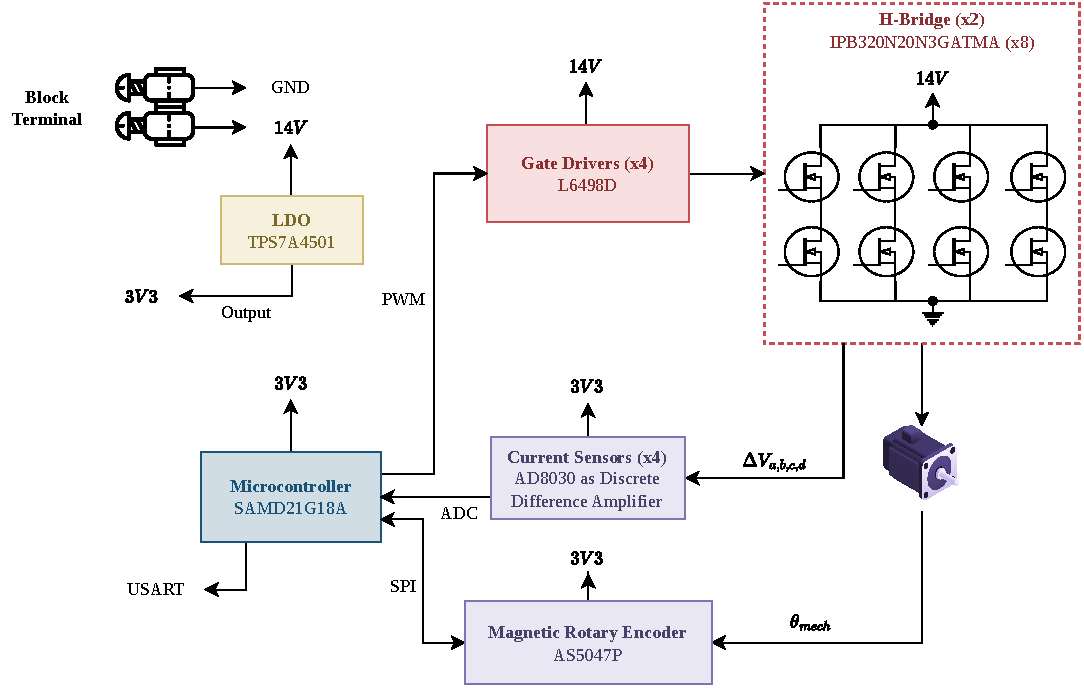
\includegraphics[width=\textwidth,keepaspectratio]{04_DesignForRadiationEnvironment/images/FirstIterationSystem.pdf}
  \caption{The high-level schematics of the first prototype system.}
  \label{fig:first-pcb-system-architecture}
\end{figure}

The board design files, including the Altium project files and associated manufacturing specifications, are available through the CERN EDMS under project \textit{EDA-05226-V1-0 v.0}.\footnote{\url{https://edms.cern.ch/ui/\#!master/navigator/item?P:101857775:101857776:subDocs}}

\begin{figure}[H]
    \centering

    \begin{subfigure}{0.49\textwidth}
        \centering
        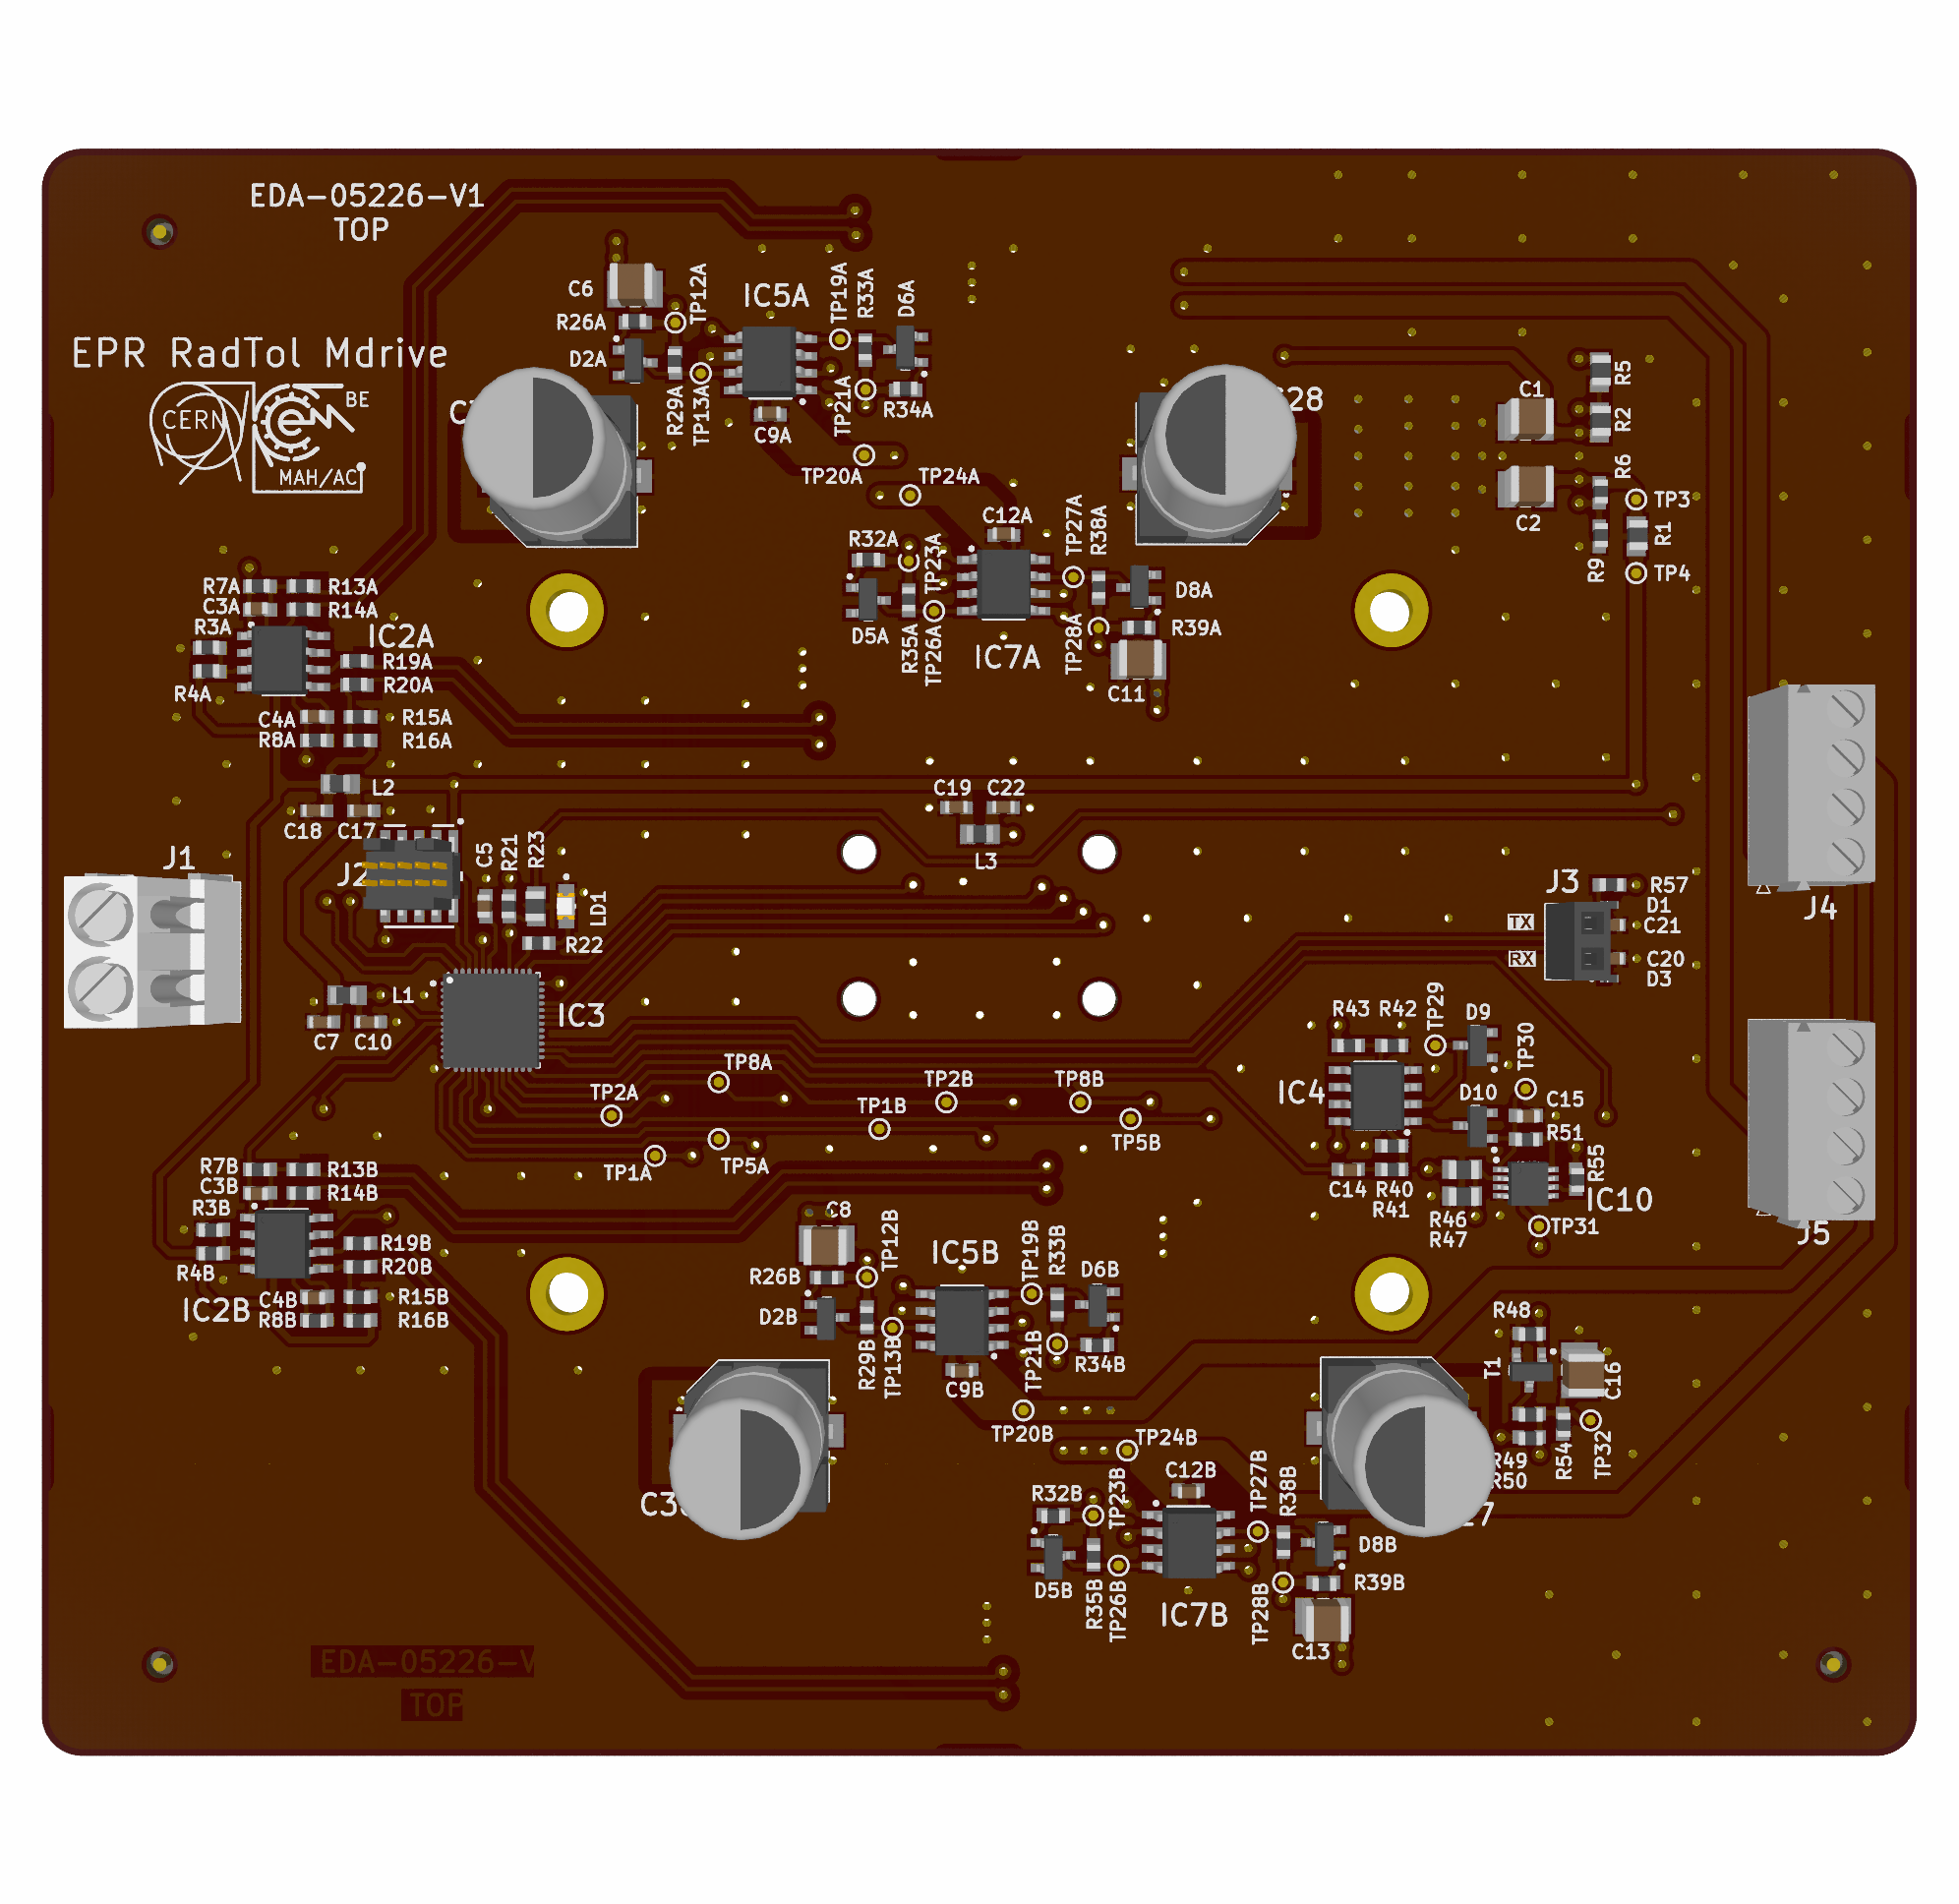
\includegraphics[width=\textwidth]{04_DesignForRadiationEnvironment/images/EDA-05226-V1-0_Front.png}
        \caption{Front side}
        \label{fig:pcb-iter-1-front}
    \end{subfigure}
    \hfill
    \begin{subfigure}{0.49\textwidth}
        \centering
        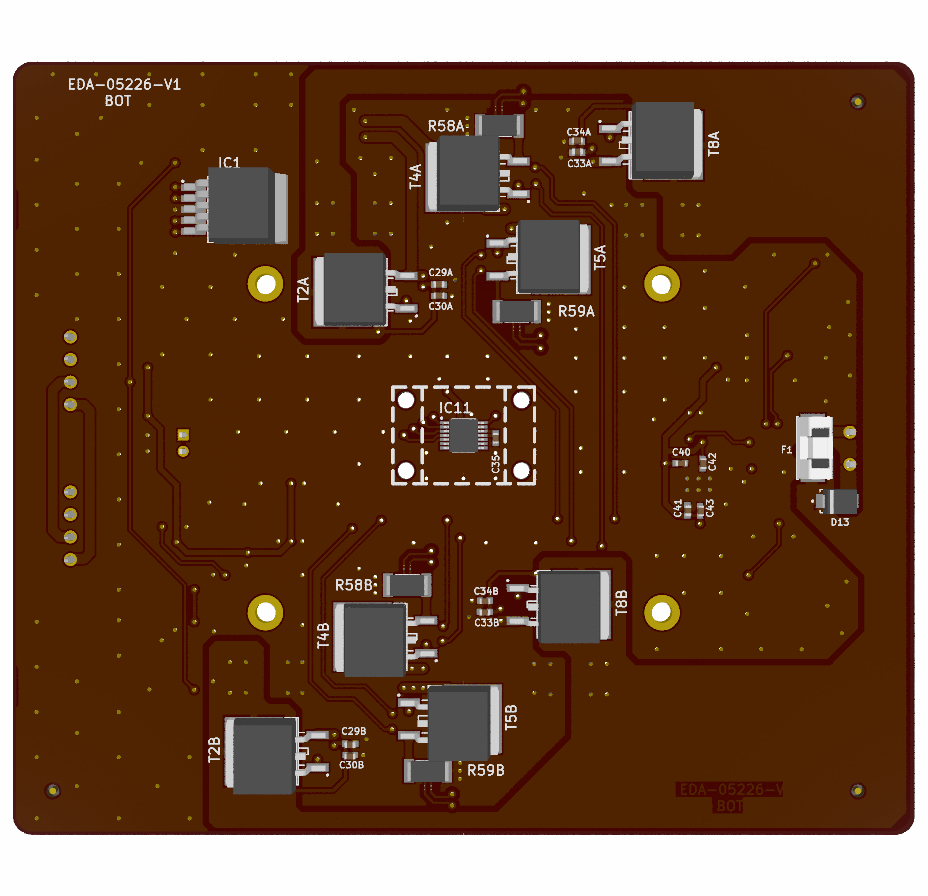
\includegraphics[width=\textwidth]{04_DesignForRadiationEnvironment/images/EDA-05226-V1-0_Back.png}
        \caption{Back side}
        \label{fig:pcb-iter-1-back}
    \end{subfigure}

    \caption{3D render of the first iteration prototype PCB, generated using the KiCad 10.0 render tool with ray tracing enabled}
    \label{fig:3d-render-pcb-iter-1}
\end{figure}

\subsection{Rad-Tol Motor Controller - Iteration 2}
\label{subsec:pcb-iter-2}
This section presents the second and most significant iteration of the radiation-tolerant motor controller. The design was fully revised based on the experience gained from the first prototype, with the most notable changes being:

\begin{itemize}
    \item The power supply was split into three separate rails — 5,V, 12,V, and 20,V — to improve observability and fault isolation during testing.
    \item An LDO was added to step down the 5,V rail to 3.3,V for the digital circuits, later replaced with a more compact part with stronger design heritage from BatMon and DIOT.
    \item The discrete difference amplifier was replaced with the INA214 integrated current-shunt amplifier, which carries RaToPUS heritage.
    \item A dedicated voltage reference IC was added to provide a stable offset voltage for the current-sense amplifier, replacing the resistor-divider approach.
    \item An external bootstrap diode was included to make the PCB compatible with both the L6498D and NCP5183 gate drivers.
    \item An external watchdog IC was added, based on BatMon heritage.
\end{itemize}

The high-level architecture and the final 3D render are shown in Figures~\ref{fig:final-pcb-system-architecture} and~\ref{fig:final-pcb-3d-render}, respectively. The implemented setup is presented in Subsection~\ref{subsubsection:fully-assembled-system} of Chapter~\ref{chapter:test-bench-design}.

\begin{figure}[H]
  \centering
  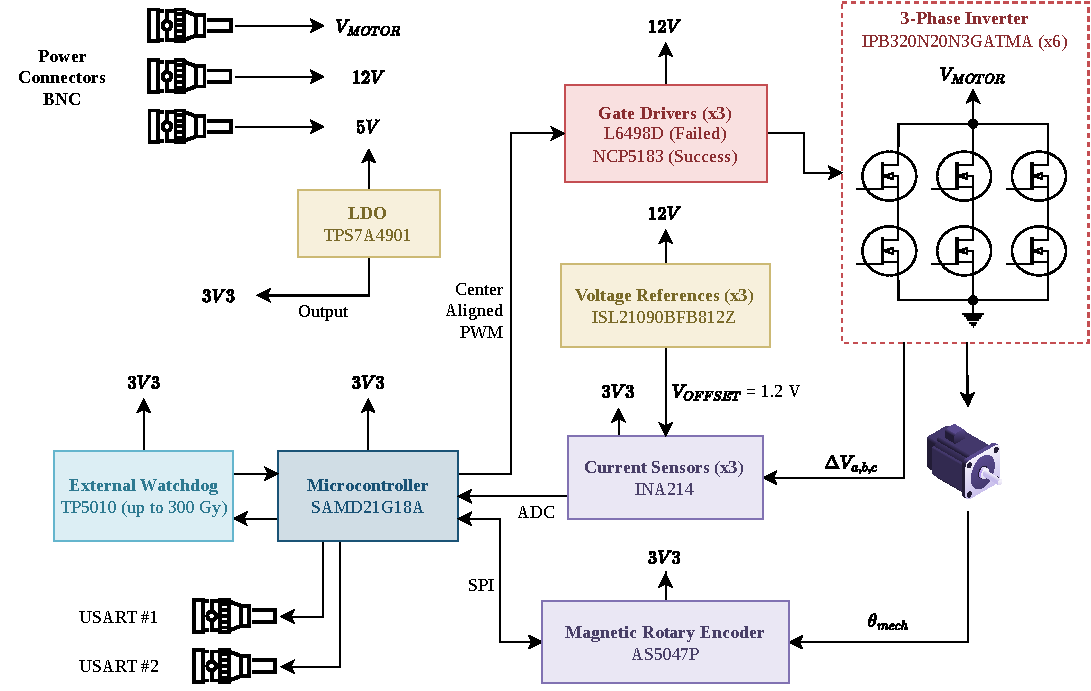
\includegraphics[width=\textwidth,keepaspectratio]{04_DesignForRadiationEnvironment/images/SecondIterationSystem.pdf}
  \caption{The high-level schematics of the final system including the critical interconnections.}
  \label{fig:final-pcb-system-architecture}
\end{figure}

\begin{figure}[H]
  \centering
  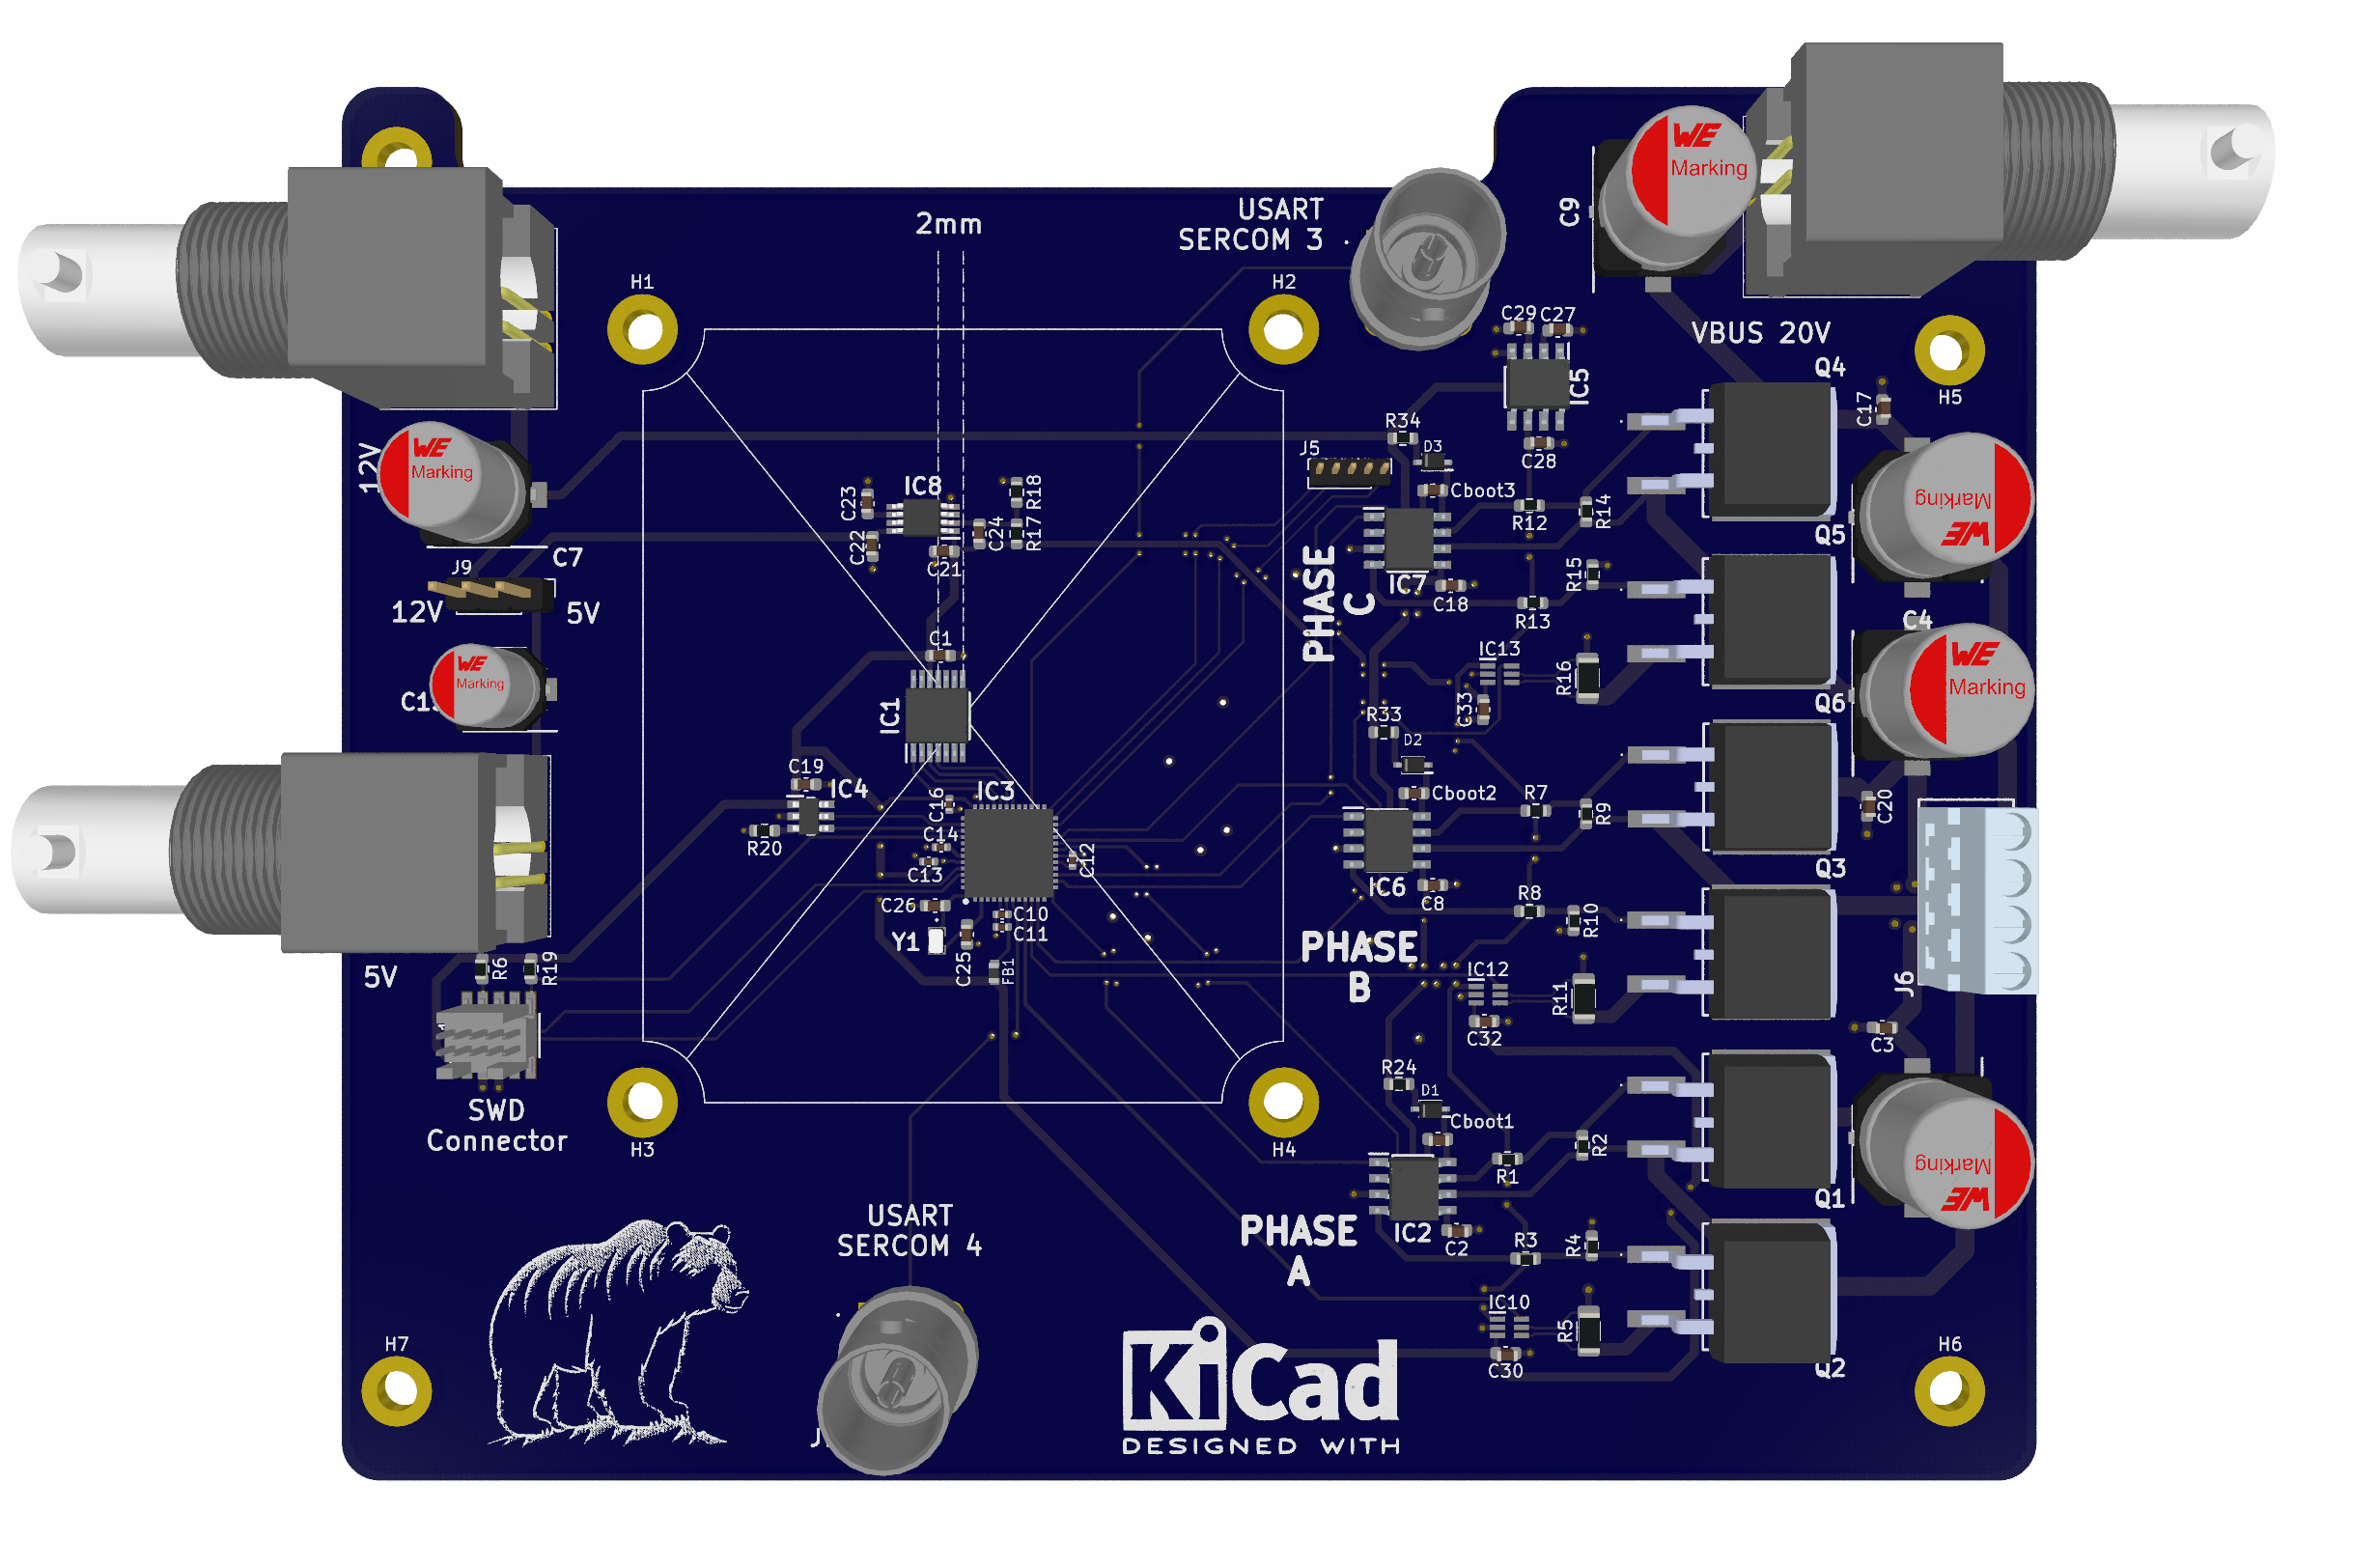
\includegraphics[width=\textwidth,keepaspectratio]{04_DesignForRadiationEnvironment/images/BLDC_Motor_Driver.png}
  \caption{The final PCB 3D using built-in KiCad 9.0 render tool with raytracing}
  \label{fig:final-pcb-3d-render}
\end{figure}

\section{Firmware Design \& Implementation}
\label{section:firmware}
A complete Field-Oriented Control (FOC) firmware stack was developed from scratch, as existing implementations were found unsuitable for the constraints of this work. FOC is a real-time control algorithm that depends on hardware-acquired physical quantities — phase currents and rotor position — and requires deterministic execution of the control loops. Existing open-source solutions such as ODrive and VESC target higher-performance architectures, while SimpleFOC's reliance on the Arduino API makes it incompatible with the low-level peripheral timing and deterministic interrupt execution required here.

A fully custom implementation was therefore developed, motivated by four main considerations:

\begin{itemize}
    \item \textbf{Performance:} The current-control loop must execute within strict real-time limits while supporting additional monitoring and fault-mitigation logic required during radiation testing.
    \item \textbf{Portability:} The control logic is kept separate from the hardware abstraction layer to allow future migration to a different MCU or an FPGA-based implementation.
    \item \textbf{Scalability:} The architecture accommodates future extensions such as alternative motor types, velocity estimators, sensing hardware, and diagnostic peripherals.
    \item \textbf{Observability:} A custom implementation makes firmware behavior easier to inspect, instrument, and analyze during radiation-induced fault events.
\end{itemize}

Low-level peripheral drivers were generated using Microchip Harmony 3 and MPLAB MCC. The remaining firmware was written manually in C++17, using CMake as the build system, ARM GCC as the compiler and linker toolchain, and OpenOCD for programming and debugging.

\subsection{FOC Implementation on the SAMD21 MCU}

As discussed previously, FOC must satisfy hard real-time requirements. The innermost current-control loop is the most time-critical part of the algorithm and must be synchronized with the PWM carrier. In this implementation, the current loop is executed from the ADC result-ready interrupt, immediately after the phase-current samples have been acquired.

To obtain fresh current measurements at the correct instant of the PWM cycle, the SAMD21 event system is used. The TCC0 peripheral generates the three-phase PWM waveform, while its fourth compare channel is configured as a hardware sampling trigger, avoiding software-trigger jitter and ensuring that the current samples are consistently acquired at the selected point of the PWM period. Once both ADC channels have been sampled, the interrupt converts the raw measurements into phase currents, executes the current-control routine, computes the new SVPWM duty cycles, and writes the updated values to the TCC0 registers, creating a deterministic chain from PWM generation to current sampling to duty-cycle update.

The SAMD21 ADC does not support simultaneous sampling, meaning the phase currents cannot be acquired at the same instant. From testing, sampling all three phase currents within a single PWM period proved infeasible due to conversion overhead. For this reason, only $I_a$ and $I_b$ are sampled, and $I_c$ is derived from the three-phase current relation. The result of $I_a$ is stored upon completion of the first conversion, after which a second conversion is triggered in software. When $I_b$ becomes available, the innermost control block executes. This process is depicted in Figure~\ref{fig:adc-isr}.

\begin{figure}[H]
  \centering
  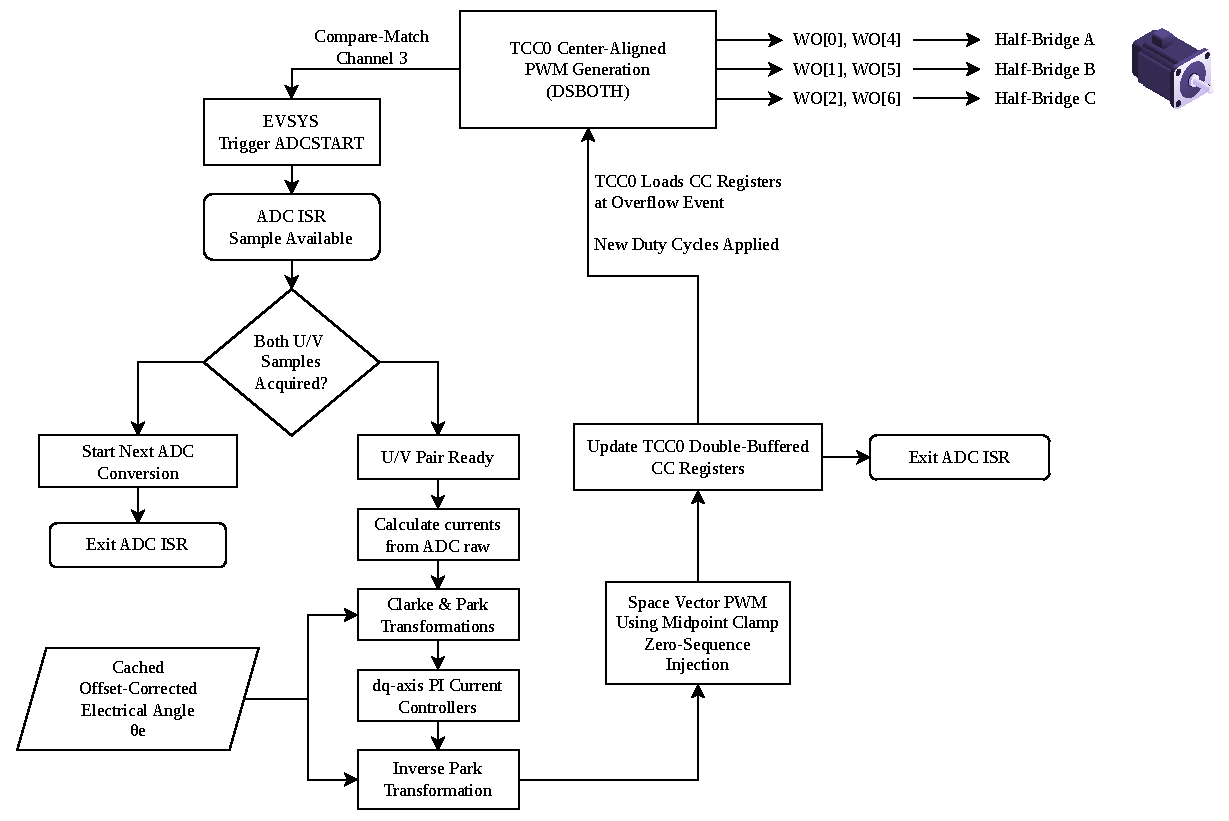
\includegraphics[width=\textwidth,keepaspectratio]{04_DesignForRadiationEnvironment/images/ADC_ISR.pdf}
  \caption{FOC current control loop execution flow inside the ADC ISR.}
  \label{fig:adc-isr}
\end{figure}

The described implementation constitutes the inner current control loops running at PWM rate. The velocity and position control loops are less time-critical and are executed by a dedicated Timer/Counter peripheral instance at a lower rate of \SI{3}{\kilo\hertz}. Due to CPU load constraints, the rotor angle $\theta_m$ --- and consequently the electrical angle $\theta_e$ --- is read at this lower rate rather than at the PWM rate.

For the communication with the SPI interface of the AS5047P magnetic encoder, a device driver was implemented in C++. Such an approach was followed in order to isolate the AS5047P logic, calculations and error handling from the HAL and enhance maintainability and portability. The sensor itself offer many protocols for reading the angle (PWM, UVW, SPI) and can only be configured through SPI. Furthermore, the driver is implemented in non-blocking/interrupt mode and not blocking, thus there are callbacks functions defined in order to be passed to the SPI Read interrupt handler.

\subsection{Compile-Time Computations \& Startup Calibration}

One of the main reasons that C++ was preferred is for its ability to perform calculations at compile time with constexpr and consteval. This is particularly useful in FOC as it contains calculations that are necessary to happen at compile time. For specifically, at the beginning of the software, there is an initialization and calibration routine that has to run. This includes the calculation of the trigonometric LUTs and their storage into flash memory and the alogirithmic zero offset electrical angle calculation and the direction calibration. Those are described in chapter \ref{chapter:motor-control-selection} as well.

\textbf{Compile-Time LUT Computation} \\
The LUTs for sine and cosine are calculated at compile time and then written directly in Flash and optionally can be copied in sram during startup. For the tests the LUTs remained in flash for safety as the corruption of sequential data would be unacceptable for the control stability.

Since the C++20 standard that is used does not support \texttt{constexpr} functions of the \texttt{<cmath>} library, an external open-source library is utilized, and more specifically the GCE-Math library~\cite{ohara_gcem}.

Due to the absence of FPU in the specific MCU, Q15 fixed-point arithmetic was used for minimum CPU overhead in computations. Furthermore, C++ zero-overhead features such as operator overloading, provide an elegant way to read from the LUT which is an \texttt{std::array} by feeding either the angle in mrad or in raw 14-bit which is the format that AS5047P magnetic encoder uses.

\textbf{Startup Calibration} \\
This runs before the actual FOC commutation and is a state machine that sequentially aims to find the zero offset electrical angle and also characterize the direction as CW or CCW so that physically changing the order of the phases of the motor does not lead to different motion.

\subsection{Radiation-Induced Faults Mitigation Attempts}

As already discussed, radiation can induce SEEs in the MCU, degrading or disrupting motor control. The approach taken is to first characterize the symptoms of unmitigated radiation-induced controllability loss, then implement and evaluate mitigation techniques accordingly.

Loss of controllability can originate from several event types, the most straightforward being a SEFI that renders the MCU non-functional. A watchdog timer (WDT) is therefore a natural mitigation measure. Since the internal WDT of the SAMD21 was found to lack radiation tolerance beyond \SI{100}{\gray}, an external WDT is introduced in the second hardware iteration. In the first iteration, this functionality is substituted by the control room PC running the telemetry and instrumentation software.


\textbf{Software Triple-Modular Redundancy}

Although TMR is most effective when implemented in hardware (e.g.\ in FPGAs, where triplicated voters can be implemented with guaranteed isolation), software reliability techniques such as N-version programming offer a viable alternative. With N-version programming, a single process is replicated into $N$ identical parallel instances, and the output is determined by a voter, as shown in Figure~\ref{fig:N-version-programming}.

\begin{figure}[H]
  \centering
  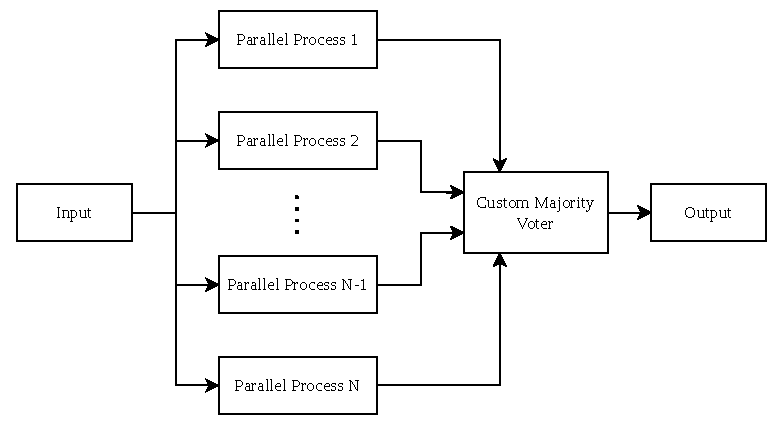
\includegraphics[width=0.8\textwidth,keepaspectratio]{04_DesignForRadiationEnvironment/images/N-version.pdf}
  \caption{N-version programming software reliability technique.}
  \label{fig:N-version-programming}
\end{figure}

Since the MCU does not support multi-threading and an RTOS would impose prohibitive performance overhead, the adopted technique is a software TMR that stores critical runtime variables in three separate RAM regions. These include algorithm parameters such as the zero-offset electrical angle and the direction variable, as well as state machine state variables. A key requirement is that the three copies are placed sufficiently far apart in memory so that a single SEU-affected memory block does not corrupt adjacent copies. This is achieved through the linker script and startup code, where three dedicated memory sections are declared with a guaranteed separation of 4096 bytes. The resulting RAM layout is illustrated in Figure~\ref{fig:samd21-ram-layout}.

The stack is placed at the beginning of the memory region so that a stack overflow triggers a hard-fault handler callback, allowing the event to be detected and logged rather than causing silent corruption.

Instead of reading a single instance of a critical variable, three copies are read and a majority voter is applied to determine the valid value. This inevitably increases code size, so the number of variables designated as critical must be kept reasonable. The process is illustrated in Figure~\ref{fig:tmr-voter}. Additionally, the breadcrumb technique is employed to store diagnostic information in non-volatile memory, enabling post-reset analysis of the fault that caused the MCU to reset.


\begin{figure}[H]
  \centering
  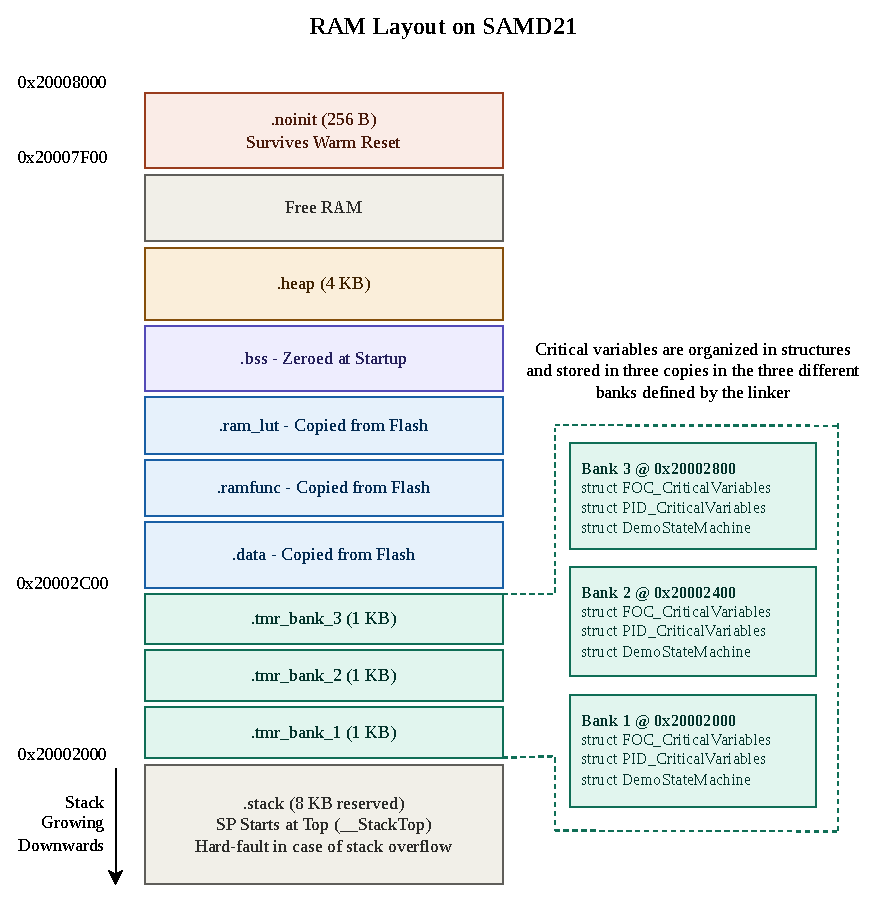
\includegraphics[
    width=0.8\textwidth,
    height=\textheight,
    keepaspectratio
  ]{04_DesignForRadiationEnvironment/images/SAMD21_RAM.pdf}
  \caption{Configured SRAM layout of the SAMD21 MCU}
  \label{fig:samd21-ram-layout}
\end{figure}

\begin{figure}[H]
  \centering
  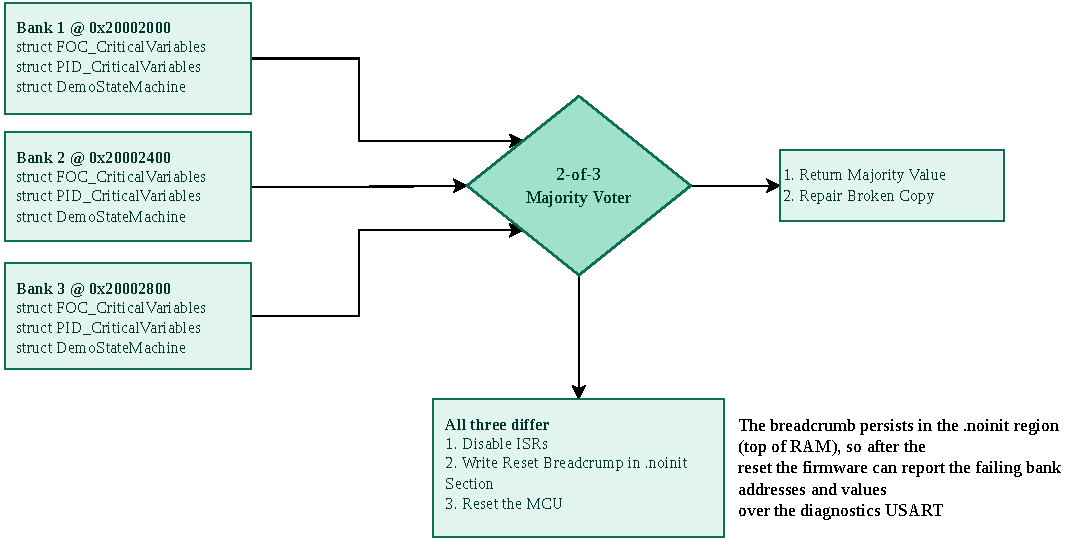
\includegraphics[
    width=\textwidth,
    height=\textheight,
    keepaspectratio
  ]{04_DesignForRadiationEnvironment/images/SAMD21_RAM_TMR.pdf}
  \caption{Reading three copies of a variable and performing TMR}
  \label{fig:tmr-voter}
\end{figure}
